\documentclass{article}
\usepackage{ctex}
\usepackage[utf8]{inputenc}
%\usepackage{natbib}
\usepackage[square,sort,comma,numbers]{natbib}
\usepackage{graphicx}
\usepackage{geometry}
\usepackage{booktabs}
\usepackage{siunitx}
\usepackage{listings}
\usepackage{subfigure}
\usepackage{appendix}
\usepackage{graphicx}
\usepackage{pythonhighlight}
\usepackage{bm}
\usepackage{makecell}
\lstset{
    language=MATLAB,
    basicstyle=\ttfamily\small,
    aboveskip={1.0\baselineskip},
    belowskip={1.0\baselineskip},
    columns=fixed,
    extendedchars=true,
    breaklines=true,
    tabsize=4,
    prebreak=\raisebox{0ex}[0ex][0ex]{\ensuremath{\hookleftarrow}},
    frame=lines,
    showtabs=false,
    showspaces=false,
    showstringspaces=false,
    keywordstyle=\color[rgb]{0.627,0.126,0.941},
    commentstyle=\color[rgb]{0.133,0.545,0.133},
    stringstyle=\color[rgb]{01,0,0},
    numbers=left,
    numberstyle=\small,
    stepnumber=1,
    numbersep=10pt,
    captionpos=t,
    escapeinside={\%*}{*}
}


\geometry{a4paper,centering,scale=0.8}
\usepackage[format=hang,font=small,textfont=it]{caption}
\usepackage[nottoc]{tocbibind}
\usepackage{float}
\usepackage{amsmath}
\usepackage[colorlinks=true, 
    linkcolor=blue,          % color of internal links
    citecolor=blue,        % color of links to bibliography
    filecolor=blue,      % color of file links
    urlcolor=blue]{hyperref}
    \usepackage[myheadings]{fullpage}

\numberwithin{equation}{subsection}
\newcommand{\HRule}[1]{\rule{\linewidth}{#1}}
\newcommand\degree{^\circ}
\date{}
%\bibliographystyle{plain}
\usepackage{abstract}
\setlength{\abstitleskip}{0em}%“摘要”与摘要正文间距
\renewcommand{\abstractnamefont}{\Large\bfseries}
\pagestyle{plain}
\geometry{a4paper,left=3cm,right=3cm}

%=================================================================
\title{\heiti 基于蒙特卡洛和粒子群遗传算法的\\定日镜场的优化设计}


\begin{document}
\maketitle
\vspace{-5em}%“摘要”与标题的间距

\begin{abstract}
塔式太阳能光热发电是一种低碳环保的新型清洁能源技术,通过定日镜将太阳光反射汇聚到吸收塔顶端的集热器,加热其中的导热介质,从而实现太阳能到热能到电能的转化输出。
定日镜场对太阳光的反射汇聚是一个复杂的过程,受到定日镜尺寸、位置、数目等多种因素的影响,并伴随着各种光学效率的损失。实现定日镜场的优化设计,对于构建以新能源为主体的
新型电力系统,实现“碳达峰”“碳中和”目标具有重要意义。 

\textbf{针对问题一:}
我们构建了太阳方位确定模型,通过计算不同时刻的太阳方位角和太阳高度角可以确定太阳入射光线的方向向量,从而根据定日镜追踪太阳位置的原理确定定日镜的镜面法向量。
为了计算定日镜的阴影遮挡效率与集热器截断效率,我们采用光线追踪法(均匀采样的蒙特卡洛法)进行建模,并构建了相应的判别器来判断选取得随机光线是否会被阴影遮挡/集热器截断。
用未被遮挡/截断的光线数目除以总光线数目可得阴影遮挡效率和集热器截断效率,综合运算后得到各定日镜的光学效率。再结合题目附录中的公式求得一年中不同时刻的功率数据(12*5=60组),
先将每日不同时间的数据取平均,再将每年不同日期的数据取平均,得到所求的年平均功率数据如表3,表4所示。

%构建浮子与振子垂荡时的物理模型。依据附件3和附件4提供的数据,结合附件1中波浪能装置的运动状态,分(1)与(2)两种情况分别对浮子与振子竖直方向上的运动进行受力分析。根据牛顿第二定律列出浮子与振子垂荡过程中的运动学\textbf{微分方程},通过换元整理转化为一阶显式常微分方程组。进而利用matlab中的\verb|odefun|函数求解微分方程的数值解,得到前40个波浪周期内时间间隔为$0.2s$的垂荡位移与速度。

\textbf{针对问题二:}
考虑到参数数目过多会导致运算量过大,我们先采用了Campo方法布置初始镜场简化参数,再使用PSO-GA(粒子群遗传算法)进行优化。考虑到镜子与塔的距离限制,我们将Campo初始镜场设置为4个紧密嵌套的同心圆环区域。所有区域内的定日镜尺寸、高度均相同,同一区域各行上的定日镜数量相同,定日镜之间最密集排布。
继而使用遗传算法与粒子群优化相结合的PSO-GA算法进行优化,优化目标为:单位镜面面积年平均输出热功率尽量大;优化限制为:年平均输出热功率大于等于 $ 60 MW$,$100m\leq$镜与塔的距离$\leq 350m$。
对于 PSO-GA 优化后的结果,按照光学效率从低到高的顺序分批剔除镜点,直至镜场的年平均输出功率大于等于 $60M W$ ,且继续剔除一个镜点会使镜场年平均输出功率小于 $60M W$ 为止。
剔除处理后得到的定日镜和集热塔坐标储存在附件result2.xlsx中,计算整理得优化镜场参数如表6,表7,表8所示。


%在问题一垂荡位移与速度的建模基础上,利用附件3和附件4中参数数值,求得特定直线阻尼器阻尼系数下垂荡过程的相对位移与相对速度。将平均输出功率视为20个波浪周期至40个波浪周期内阻尼力做功量与用时的比值。而一段时间的做功量等于阻尼力对时间的积分,利用数值方法将其近似为微小梯形面积之和。(1)对于给定的较小步长,将直线阻尼系数在[0,100000]\textbf{遍历}(2)对于给定的较小的步长,将系数与幂指数在分别在[0,100000]与[0,1]之间\textbf{遍历}。得到平均输出功率的数据散点图,并通过最大值点的检索和估计,得到最大平均输出功率和对应阻尼系数。

\textbf{针对问题三:}
相较于问题二,问题三引入了更多可以优化的参数,但同样适用问题二的Campo初始镜场布置-PSO-GA优化-剔除低效镜点模型。
将初始镜场设置为4个紧密嵌套的同心圆环区域,同一区域内的定日镜尺寸、高度相同,不同区域内的定日镜尺寸、高度可以不同,同一区域各行上的定日镜数量相同,定日镜之间最密集排布。
对简化后的镜场参数采用PSO-GA混合算法进行优化并分批分批剔除镜点,优化目标、优化限制以及低效镜点提出原则与问题二相同。
处理后得到的定日镜和集热塔尺寸及坐标储存在附件result3.xlsx中,计算整理得优化镜场参数如表10,表11,表12所示。
%构建浮子与振子垂荡纵摇时的物理模型。通过假定浮子的旋转轴以及其旋转轴心处的运动状态,利用附件3和附件4提供的数据,对浮子和振子在垂荡运动方向与纵摇旋转方向上进行受力分析。模型求解思路同问题一,将得到的运动方程化为一阶显式微分方程组后,进利用matlab中的\verb|odefun|函数求解微分方程的数值解,得到前40个波浪周期内时间间隔为$0.2s$的浮子与振子垂荡位移与速度、纵摇角位移与角速度。

最后,我们对问题1中结论数据进行了多项式插值,观察得到的“日期-时间-参量”曲面图。曲面的变化较为平缓,说明光线追迹的蒙特卡洛算法灵敏度较低,模型稳定性很好。 

\textbf{关键词:光线追迹;蒙特卡洛;Campo布置;PSO-GA算法}

\end{abstract}

\newpage

%=================================================================

{\centering\section{问题重述}}

\subsection{问题背景}
塔式太阳能光热发电是一种低碳环保的新型清洁能源技术,对于构建以新能源为主体的新型电力系统,实现“碳达峰”“碳中和”目标具有重要意义。
定日镜是塔式电站收集太阳能的基本组件,其底座由纵向转轴和水平转轴组成,平面反射镜安装在水平转轴上(图1)。纵向转轴的轴线与地面垂直,控制反射镜的方位角;水平转轴的轴线与地面平行,控制反射镜的俯仰角。
塔式电站利用大量的定日镜组成阵列,称为定日镜场。定日镜将太阳光反射汇聚到安装在镜场中吸收塔顶端上的集热器,加热其中的导热介质,并将太阳能以热能形式储存,再经过热交换实现由热能向电能的转化。
定日镜在工作时,控制系统根据太阳的位置实时控制定日镜的法向,使得太阳中心点发出的光线经定日镜中心反射后指向集热器中心。
\begin{figure}[htbp]
	\begin{minipage}{0.4\linewidth}
		\centering
		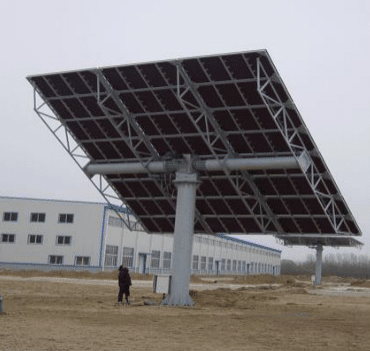
\includegraphics[width=1.8in]{定日镜及底座示意图.png}
		\caption{定日镜及底座示意图}
	\end{minipage}
	\begin{minipage}{0.5\linewidth}
		\centering
		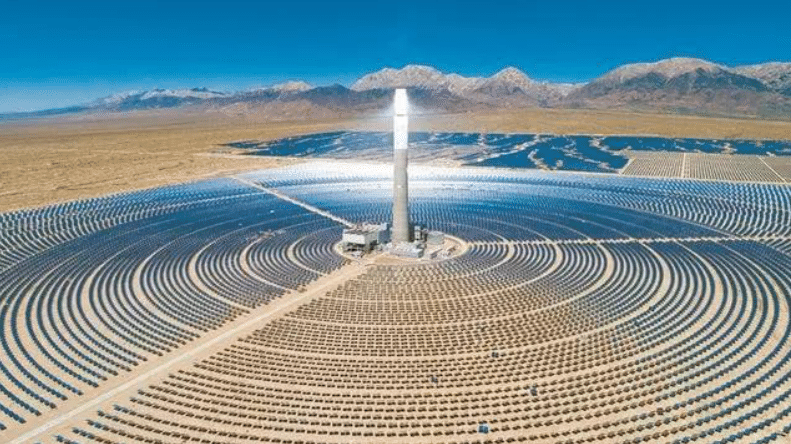
\includegraphics[width=3.08in]{圆形定日镜场示意图.png}
		\caption{圆形定日镜场示意图}
	\end{minipage}
\end{figure}

\subsection{目标任务}
现计划在中心位于东经$98.5°$,北纬$39.4°$,海拔$3000m$,半径$350m$的圆形区域内建设一个圆形定日镜场(图 2)。以圆形区域中心为原点,正东方向为$x$轴正向,正北方向为$y$轴正向,垂直于地面向上方向为$z$轴正向建立坐标系,称为镜场坐标系。
规划的吸收塔高度为$80m$,圆柱形外表受光式集热器高$8m$,直径$7m$,平面矩形定日镜边长在$2m$到$8m$之间,安装高度在$2m$至$6m$之间。安装要求吸收塔周围$100m$范围内不安装定日镜,相邻定日镜底座中心之间的距离比镜面宽度多$5m$以上。
为简化计算,本问题中所有“年均”指标的计算时点均为当地时间每月 21 日 9:00、10:30、12:00、13:30、15:00,据此建立模型并解决以下问题:

\textbf{问题1:}给定吸收塔与定日镜位置如附件所示。定日镜尺寸$6m\times 6m$,安装高度$4m$。计算该定日镜场的年平均光学效率、年平均输出热功率,以及单位镜面面积年平均输出热功率。

\textbf{问题2:}若所有定日镜尺寸及安装高度相同,设计定日镜的尺寸、安装高度、数目,以及吸收塔与定日镜的位置坐标参数,使得定日镜场达到额定年平均输出功率$60MW$的条件下,单位镜面面积年平均输出热功率尽量大。

\textbf{问题3:}若定日镜尺寸及安装高度可以不同,设计定日镜场的各个参数,使得定日镜场达到额定年平均输出功率$60MW$的条件下,单位镜面面积年平均输出热功率尽量大。

%-------------------------------------------------------------------
{\centering\section{问题分析}}

\subsection{问题一的分析}
问题一给定了定日镜场的各个参数,要求计算该镜场的年平均光学效率、年平均输出热功率和单位镜面面积年平均输出热功率。
首先我们求解了一年中不同时刻的太阳方位角和太阳高度角,确定太阳入射光线的方向向量,从而根据定日镜追踪太阳位置的原理确定定日镜的镜面法向量。
由于定日镜的阴影遮挡现象和集热器截断现象是两个复杂的过程,我们采用了光线追迹法(均匀采样的蒙特卡洛法)进行建模,并构建了相应的判别器来判断选取得随机光线是否会被阴影遮挡/集热器截断。
用未被遮挡/截断的光线数目除以总光线数目可得阴影遮挡效率和集热器截断效率,
综合运算后得到各定日镜的光学效率。再结合题目附录中的公式求得一年中不同时刻的功率数据(12*5=60组),先将每日不同时间的数据取平均,再将每年不同日期的数据取平均,得到所求的年平均功率数据。

\subsection{问题二的分析}
问题二要在定日镜尺寸和安装高度相同的前提下设计镜场参数,使得镜场达到额定功率且单位镜面面积年平均输出热功率尽量大。
考虑到参数数目过多会导致运算量爆炸,我们采用Campo布置方法\cite{7}对参数进行了简化:
将初始镜场设置为4个紧密嵌套的同心圆环区域,所有区域内的定日镜尺寸、高度均相同,同一区域各行上的定日镜数量相同,定日镜之间最密集排布。
在此基础上,我们对简化后的镜场参数采用PSO-GA混合算法进行优化。综合了遗传算法(GA)和粒子群优化(PSO)的优点,PSO-GA具有更好的综合表现。\cite{8}
优化目标为:单位镜面面积年平均输出热功率尽量大;优化限制为:年平均输出热功率大于等于 $ 60 MW$,$100m\leq$镜与塔的距离$\leq 350m$。
考虑到圆环形的初始镜场中极有可能存在低效率的镜点,拉低了镜场的单位镜面面积年平均输出热功率。因此对于 PSO-GA 优化后的结果,按照光学效率从低到高的顺序分批剔除镜点,
直至镜场的年平均输出功率大于等于 $60M W$ ,且继续剔除一个镜点会使镜场年平均输出功率小于 $60M W$ 为止。
剔除处理后得到的数据即为所求的优化镜场参数。

%问题二分析内容
\subsection{问题三的分析}
问题三要在定日镜尺寸和安装高度可以不同的条件下设计镜场参数,使得镜场达到额定功率且单位镜面面积年平均输出热功率尽量大。
相较于问题二,问题三引入了更多可以优化的参数,但同样适用问题二的Campo初始镜场布置-PSO-GA优化-剔除低效镜点模型。
将初始镜场设置为4个紧密嵌套的同心圆环区域,同一区域内的定日镜尺寸、高度相同,不同区域内的定日镜尺寸、高度可以不同,同一区域各行上的定日镜数量相同,定日镜之间最密集排布。
对简化后的镜场参数采用PSO-GA混合算法进行优化并分批分批剔除镜点,优化目标、优化限制以及低效镜点提出原则与问题二相同。
处理后得到的数据即为所求的优化镜场参数。


%========================================================
\newpage

{\centering\section{模型假设}}

\begin{enumerate}
    \item 在定日镜场内,不考虑太阳光入射角和方位角的微小变化。
    \item 考虑阴影遮挡效率时,集热塔的阴影近似为矩形。 
    \item 考虑阴影遮挡效率时,太阳光看做一族平行的光线入射且按照入射方向均匀分布。
    \item 考虑集热器截断效率时,不再考虑其他镜面对太阳光锥的阻挡。
    \item 考虑集热器截断效率时,假设太阳光锥光能按照半角展宽均匀分布。
    \item 考虑问题二、三时,假设按照Campo布置镜场的单位面积年平均输出热功率最大\cite{7}。
\end{enumerate}



{\centering\section{符号说明}}

\begin{table}[H]
    \centering
    \setlength{\tabcolsep}{12mm}{ %调整表格横向宽度
    \begin{tabular}{ccc}%调整表格列数
        \toprule[1.5pt]%调节横线1粗细
        符号 & 解释 & 单位\\
        \midrule[1pt]%调节横线2粗细
        $D$&以春分作为第0天起算的天数 & -\\       
        $ST$&当地时间(24小时制) & -\\
        $\varphi$& 当地纬度&$°$ \\
        $H$& 海拔高度& $km$\\
        $\omega$& 太阳时角&$rad$ \\
        $\alpha_s$& 太阳高度角&$°$ \\
        $\gamma_s$& 太阳方位角&$°$ \\
        $\delta$& 太阳赤纬角&$rad$ \\
        $\eta_{cos}$& 余弦效率& -\\
        $\eta_{at}$& 大气透射率&- \\
        $\eta_{sb}$& 阴影遮挡效率&- \\
        $\eta_{trunc}$& 集热器截断效率&- \\
        $\eta_{ref}$& 镜面反射率(0.92)& -\\
        $G_0$& 太阳常数(1.366)&$kW/m^2$ \\
        $DNI$& 法向直接辐射辐照度&$kW/m^2$ \\
        $\eta_i$&第$i$面镜子的光学效率 &- \\
        $A_i$&第$i$面定日镜采光面积 &$m^2$ \\
        $E_{field}$&定日镜场的输出热功率 &$kW$ \\
        $\bm{n_i}$&第$i$面镜子的法向量 &-\\
        $d_{HR}$& 镜面中心到集热器中心的距离& $m$\\
        $\bm{s_i}$&第$i$面镜子入射光线的方向向量&-\\
        $\bm{t_i}$&第$i$面镜子反射光线的方向向量&-\\
        $\bm{p_{ij}}$&第$i$面镜子上选取的第$j$个点的坐标向量 &-\\
        \bottomrule[1.5pt]%调节横线3粗细
    \end{tabular}}
    \caption{符号说明(注:未申明的变量以其在出现处的具体说明为准)}
\end{table}
%三线表,符号说明
%表格具体尺寸参数调整:https://blog.csdn.net/u010158659/article/details/78964030

%=================================================================

\newpage
{\centering\section{问题一模型的建立与求解}}

\subsection{问题一模型的建立}

定日镜是用来实时追踪太阳位置并将太阳光准确地反射到集热器的光学装置。欲计算该定日镜场的年平均光学效率,首先应确定一年不同时刻太阳的方位,即太阳高度角和太阳方位角,根据太阳角度运算得到不同位置的定日镜的光学效率、采光面积等数据,从而计算该定日场年平均光学效率、年平均输出热功率,以及单位镜面面积年平均输出热功率。

\subsubsection{太阳方位的确定}

在镜场坐标系的基础上考虑太阳的运动,将太阳与坐标系原点之间的连线与地平面之间的夹角称为太阳高度角,用$\alpha_s$表示;将太阳与坐标系原点之间的连线在基础平面上的投影从北方沿着地平线顺时针量度得到的角称为太阳方位角,用$\gamma_s$表示(图3,图4)。任一时刻太阳的方位可由太阳高度角$\alpha_s$和太阳方位角$\gamma_s$这两个参数来描述。

\vskip 0.25cm
\begin{figure}[htbp]
	\begin{minipage}[b]{0.45\linewidth}
		\centering
		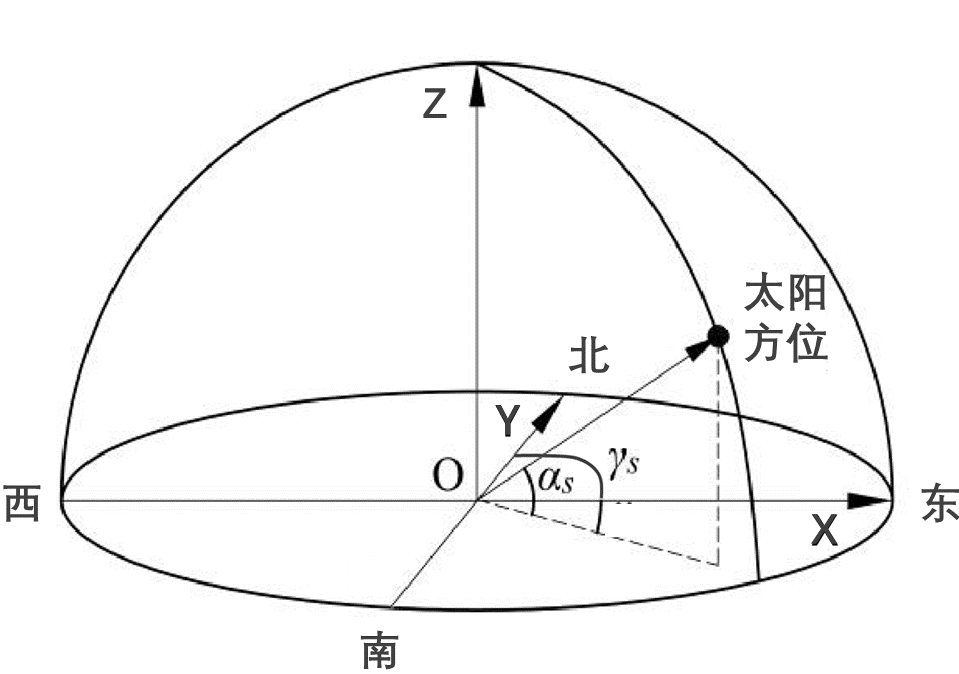
\includegraphics[width=2.4in]{问题1-1太阳方位建系图.png}
		\caption{问题1太阳方位坐标系示意图}
	\end{minipage}
	\begin{minipage}[b]{0.55\linewidth}
		\centering
		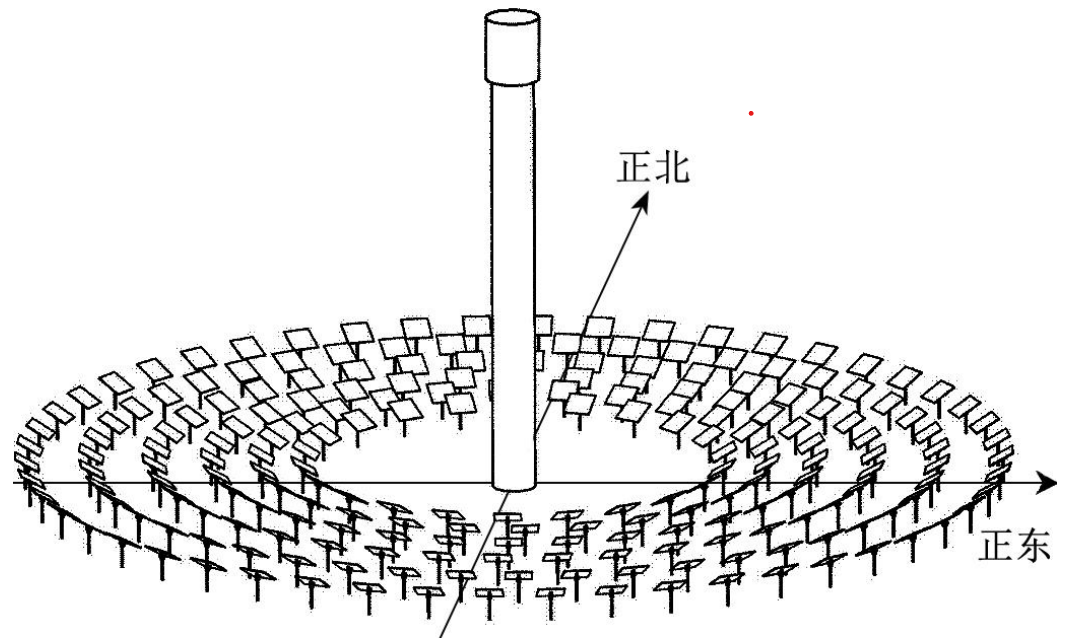
\includegraphics[width=2.6in]{问题1-1定日镜场建系图.png}
		\caption{问题1定日镜场坐标系示意图}
	\end{minipage}
\end{figure}

记当地纬度$\varphi=39.4°$,当地时间$ST$可取$9, 10.5, 12, 13.5, 15$。用$D$表示以春分(3月21日)作为第0天起算的天数,即1-12月的21日分别对应$D=0,31,61,92,122,153,184,214,245,\\275,306,337$。由题目给出的公式可知:

\begin{equation}
    \begin{aligned}
        &\text{太阳赤纬角$\delta$:}\sin \delta=\sin \frac{2 \pi D}{365} \sin \left(\frac{2 \pi}{360} 23.45\right)\\
        &\text{太阳时角$\omega$:}\omega=\frac{\pi}{12}(S T-12)\\
        &\text{太阳高度角$\alpha_s$:}\sin \alpha_s=\cos \delta \cos \varphi \cos \omega+\sin \delta \sin \varphi\\
        &\text{太阳方位角$\gamma_s$:}\cos \gamma_s=\frac{\sin \delta-\sin \alpha_s \sin \varphi}{\cos \alpha_s \cos \varphi}.\\
    \end{aligned}
\end{equation}

\vskip 0.25cm
对得到的$\sin \alpha_s$与$\cos \gamma_s$值取反三角函数,整理得60个时刻的太阳高度角$\alpha_s$和太阳方位角$\gamma_s$数据如下表所示:
\newpage
\begin{table}[!htbp]
    \centering
    \begin{tabular}{|c|c|c|c|c|c|}\hline
        $(\alpha_s,\gamma_s)$&9:00&10:30&12:00&13:30&15:00\\\hline
        1月21日&(17.43,135.78)&	(27.21,156.11)&	(30.83,180.0)&	(27.21,203.89)&	(17.43,224.22)\\
        2月21日&(24.83,130.02)&	(35.77,152.38)&	(39.97,180.0)&	(35.77,207.62)	&(24.83,229.98)\\
        3月21日&(33.12,122.4)&	(45.55,146.87)&	(50.6,180.0)	&(45.55,213.13)&	(33.12,237.6)\\
        4月21日&(41.57,112.24)&	(55.85,138.11)&	(62.28,180.0)&	(55.85,221.89)&	(41.57,247.76)\\
        5月21日&(47.05,103.1)&	(62.77,128.3)	&(70.79,180.0)	&(62.77,231.7)&	(47.05,256.9)\\
        6月21日&(48.93,99.13)&	(65.17,123.29)&	(74.05,180.0)&	(65.17,236.71)&	(48.93,260.87)\\
        7月21日&(46.99,103.23)&	(62.69,128.44)&	(70.69,180.0)&	(62.69,231.56)&	(46.99,256.77)\\
        8月21日&(41.22,112.74)&	(55.41,138.6)	&(61.76,180.0)&	(55.41,221.4)&	(41.22,247.26)\\
        9月21日&(32.67,122.86)&	(45.02,147.22)	&(50.01,180.0)&	(45.02,212.78)&	(32.67,237.14)\\
        10月21日&(23.85,130.83)&	(34.63,152.92)&	(38.75,180.0)&	(34.63,207.08)&	(23.85,229.17)\\
        11月21日&(16.83,136.21)&	(26.51,156.39)&	(30.1,180.0)&	(26.51,203.61)&	(16.83,223.79)\\
        12月21日&(14.4,137.95)&	(23.73,157.45)&	(27.16,180.0)	&(23.73,202.55)	&(14.4,222.05)\\
        \hline
    \end{tabular}
    \caption{问题1不同时刻$\alpha_s$与$\gamma_s$数据表}
\end{table}
%表格具体尺寸参数调整:https://blog.csdn.net/u010158659/article/details/78964030
%--------------------------------------------------------------------
\subsubsection{镜面法向的确定}
考虑确定不同时刻第$i$个定日镜的镜面法向量$\bm{n_i}$。
由于同一时刻所有定日镜接受到的太阳高度角$\alpha_s$和太阳方位角$\gamma_s$均相同,故每一个定日镜上的入射光线的方向向量$\bm{s_i}$相同,即:
\begin{equation}
    \bm{s_i}=\frac{1}{\sqrt{\cos^2 \alpha_s \sin^2 \gamma_s+\cos^2 \alpha_s \cos^2 \gamma_s+\sin^2 \alpha_s}}\left(
        \cos \alpha_s \sin \gamma_s ,
        -\cos \alpha_s \cos \gamma_s ,
        -\sin \alpha_s\right)
\end{equation}
由于定日镜可以实时追踪太阳位置并将太阳光准确地反射到集热器,记第$i$个定日镜的镜面中心坐标为$(x_i,y_i,z_i)$,集热器的镜面中心坐标为$(0,0,H)$,则反射光的方向向量$\bm{t_i}$为:
\begin{equation}
    \bm{t_i}=\frac{1}{\sqrt{(x_i^2+y_i^2+(z_i-H)^2)}}\left(
        -x_i,-y_i,H-z_i\right)
\end{equation}
将$\bm{t_i}$与$\bm{s_i}$相减并归一化,得到第$i$个定日镜的镜面法向量$\bm{n_i}$(图5):
\begin{equation}
    \bm{n_i}=\frac{1}{|\bm{t_i}-\bm{s_i}|}\left(\bm{t_i}-\bm{s_i}\right)
\end{equation}
\begin{figure}[H]
    \centering
    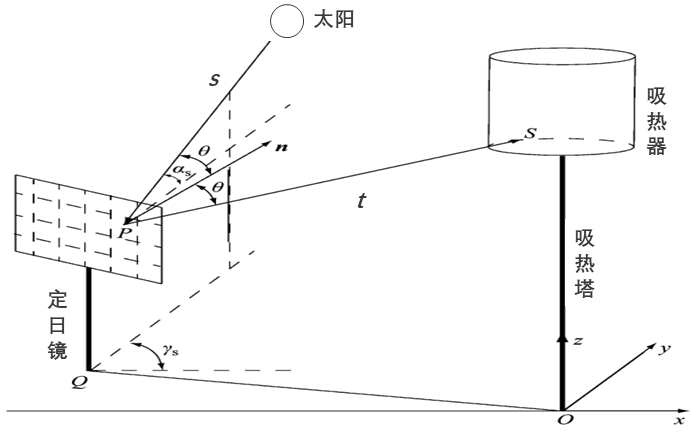
\includegraphics[scale=0.45]{问题1-1光线反射示意图.png}
    \caption{问题1太阳光线追迹示意图}
\end{figure}

\subsubsection{阴影遮挡效率}

阴影遮挡损失包括三部分\cite{3}:1.塔对镜场造成的阴影损失。
2.后排定日镜接收的太阳光被前方定日镜所阻挡造成的阴影损失。
3.后排定日镜在反射太阳光时被前方定日镜阻挡而未到达集热器上造成的遮挡损失。
本文中我们将其分为两大类:塔造成的阴影遮挡损失1和定日镜造成的阴影遮挡损失2,3。

我们采用蒙特卡洛法来计算阴影遮挡效率。对于某个固定的时刻,在每个定日镜上均匀取点,输入两个判断器分别进行以下判断:
(1)通过该点的入射光线或反射光线是否会被定日镜遮挡,是输出0,否输出1。
(2)该点是否被塔的阴影覆盖,是输出0,否输出1;
将两个判断器的输出结果相乘得到综合判断结果,若为1则说明该点不会被阴影遮挡,若为0则说明该点会被遮挡。将所有点的综合判断结果相加并除以总点数,得到定日镜阴影遮挡效率(图6)。

\begin{figure}[H]
    \centering
    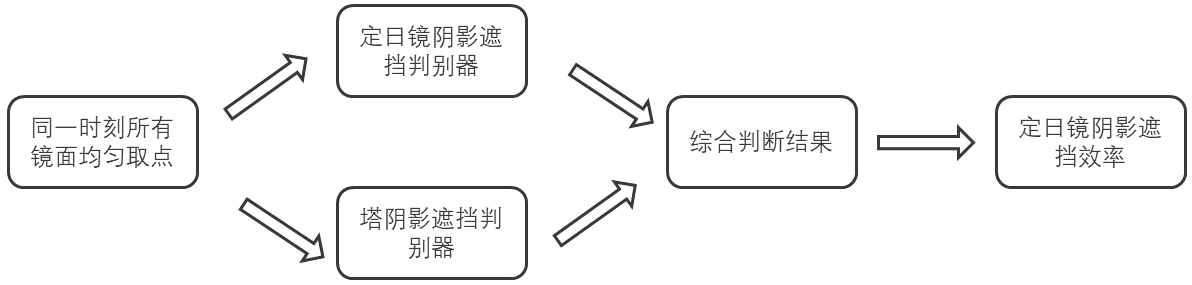
\includegraphics[scale=0.4]{问题1-1阴影遮敝率建模.png}
    \caption{问题1定日场阴影遮挡效率计算流程图}
\end{figure}

\paragraph{(1-1)定日镜阴影遮挡建模}

对于第$i$个定日镜的镜平面,以镜平面的中心为原点,以平行于镜面高的方向为$r$轴,向上为正方向,记单位向量为$\bm{r_i}$;
以平行于镜面宽的方向为$l$轴,向右为正方向,记单位向量为$\bm{l_i}$(图7)。
设第$i$个定日镜镜面中心坐标向量为$\bm{m_i}=(x_i,y_i,z_i)$,镜面法向量为$\bm{n_i}=\left(a_i,b_i,c_i\right)$,则可解$\bm{l_i},\bm{r_i}$得:
\begin{equation}
    \begin{aligned}
        &\bm{l_i}=\frac{1}{\sqrt{a_i^2+b_i^2}}\left(b_i,-ai,0\right)\\
        &\bm{r_i}=\frac{1}{\sqrt{a_i^2c_i^2+c_i^2b_i^2+(a_i^2+b_i^2)^2}}\left(a_i c_i,c_i b_i ,-a_i^2-b_i^2\right)\\
    \end{aligned}
\end{equation}

\vskip 0.25cm
\noindent
在每个定日镜上均匀取点。对于第$i$个定日镜的$l-r$坐标系,该镜面上第$j$个点的坐标向量记为$\bm{p_{ij}}=(l_{ij},r_{ij})$。
转换为定日场坐标系,该点的坐标向量为$\bm{p_{ij}}=\bm{m_i}+l_{ij}\bm{l_i}+r_{ij}\bm{r_i}$。
\begin{figure}[htbp]
	\begin{minipage}[b]{0.5\linewidth}
		\centering
		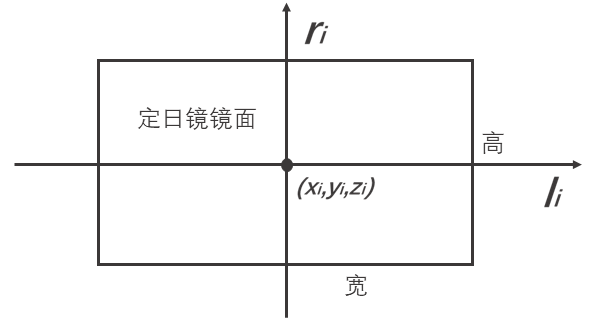
\includegraphics[width=2.6in]{问题1-1定日镜面建系图.png}
		\caption{问题1定日镜面$l-r$坐标系示意图}
	\end{minipage}
	\begin{minipage}[b]{0.5\linewidth}
		\centering
		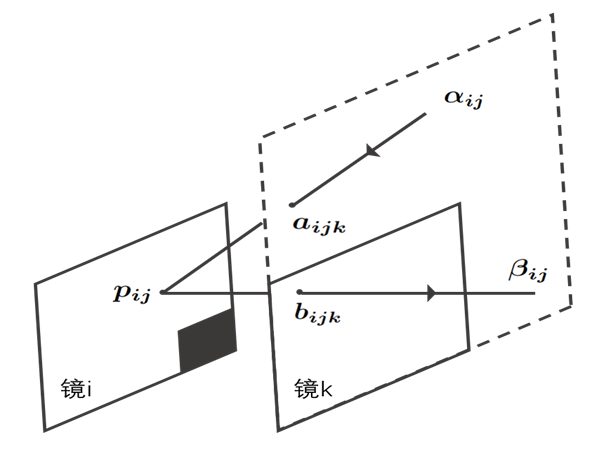
\includegraphics[width=2.4in]{问题1-1定日镜反射示意图.png}
		\caption{问题1入射反射光线与镜平面交点示意图}
	\end{minipage}
\end{figure}
\vskip 0.25cm
\noindent
已知第$i$个定日镜上入射光线与反射光线的方向向量分别为$\bm{s_i},\bm{t_i}$,设$t$为参数,则经过第$i$面定日镜上第$j$个点的入射光线向量$\bm{\alpha_{ij}}$与反射光线向量$\bm{\beta_{ij}}$可以参数化地表示为:
\begin{equation}
    \begin{aligned}
        &\bm{\alpha_{ij}}=\bm{p_{ij}}+t\,\bm{s_i}\\
        &\bm{\beta_{ij}}=\bm{p_{ij}}+t\,\bm{t_i}\\
    \end{aligned}
\end{equation}

\vskip 0.25cm
\noindent
继而考虑第$i$个定日镜旁边的第$k$个定日镜$(i\neq k)$,记第$k$个镜平面上任意一点的坐标向量为$\bm{p}$,则第$k$个镜平面的镜面方程可表示为:$\bm{n_k}\cdot (\bm{p}-\bm{m_k})=0$ 。
想要确定第$i$个镜平面上第$j$个点的入射光线或反射光线是否会与第$k$个镜平面相交,
只需求解$\bm{\alpha_{ij}},\bm{\beta_{ij}}$和无限大镜平面$\bm{n_k}\cdot (\bm{p}-\bm{m_k})=0$的交点坐标,判断交点是否在第$k$面镜子的范围内即可(图8)。

\vskip 0.25cm
\noindent
记第$i$个镜平面上第$j$个点的入射光线与第$k$个无限大的镜平面的交点坐标向量为$\bm{a_{ijk}}$,

\noindent
记第$i$个镜平面上第$j$个点的反射光线与第$k$个无限大的镜平面的交点坐标向量为$\bm{b_{ijk}}$。

\noindent
联立解得$\bm{a_{ijk}},\bm{b_{ijk}}$如下:
\begin{equation}
    \left\{\begin{array}{l}
        \bm{n_k}\cdot(\bm{p_{ij}}+t\,\bm{s_i}-\bm{m_k})=0 \quad \Rightarrow \quad \bm{a_{ijk}}=\bm{p_{ij}}+\frac{\bm{n_k}\cdot (\bm{m_k}-\bm{p_{ij}})}{\bm{n_k}\cdot \bm{s_i}} \bm{s_i}\\
        \bm{a_{ijk}}=\bm{p_{ij}}+t\,\bm{s_i}\\
    \end{array}\right.
\end{equation}
\begin{equation}
    \left\{\begin{array}{l}
        \bm{n_k}\cdot(\bm{p_{ij}}+t\,\bm{t_i}-\bm{m_k})=0 \quad \Rightarrow \quad \bm{b_{ijk}}=\bm{p_{ij}}+\frac{\bm{n_k}\cdot (\bm{m_k}-\bm{p_{ij}})}{\bm{n_k}\cdot \bm{s_i}} \bm{t_i}\\
        \bm{b_{ijk}}=\bm{p_{ij}}+t\,\bm{t_i}\\
    \end{array}\right.
\end{equation}


\paragraph{(1-2)定日镜阴影遮挡判别器}

对每一组$i,k$,构建判别器判断$\bm{a_{ijk}},\bm{b_{ijk}}$是否在第$k$面定日镜的镜子范围内。
具体判别流程如下(图9):
%$|(\bm{a_{ijk}}-\bm{m_k})\cdot \bm{l_k}| \geq $第$k$镜宽
%$|(\bm{a_{ijk}}-\bm{m_k})\cdot \bm{r_k}| \geq $第$k$镜高
%$|(\bm{b_{ijk}}-\bm{m_k})\cdot \bm{l_k}| \geq $第$k$镜宽
%$|(\bm{b_{ijk}}-\bm{m_k})\cdot \bm{r_k}| \geq $第$k$镜高
\begin{figure}[H]
    \centering
    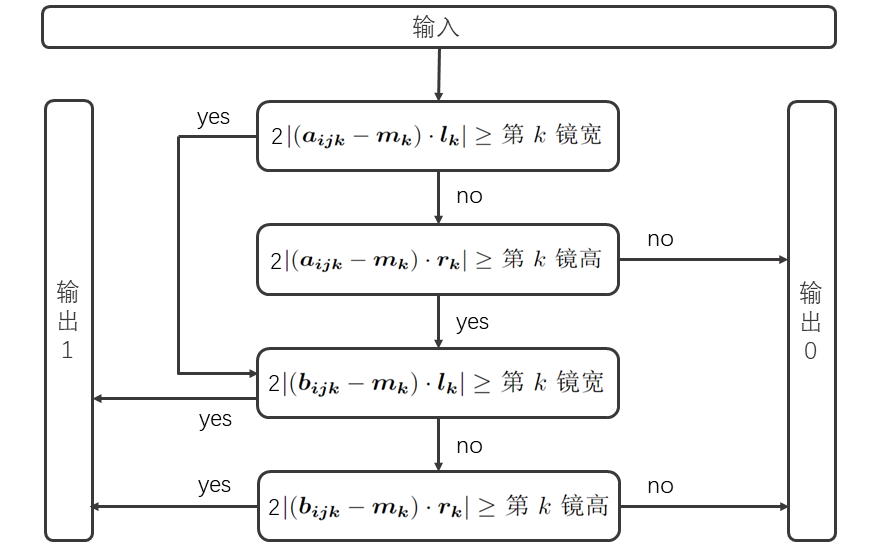
\includegraphics[scale=0.45]{问题1-1定日镜阴影遮挡判别器原理.png}
    \caption{问题1定日镜阴影遮挡判别器原理示意图}
\end{figure}

\paragraph{(2-1)塔阴影遮挡建模}

由题图可知,塔可视作半径为$\frac{7}{2}m$,高为$84m$的圆柱体。将塔的阴影近似为矩形,
以镜场坐标系的中心为原点,以太阳光在地平面上的投影方向为$r$轴,影子方向为正方向,记单位向量为$\bm{r_{\text{阴}}}$;
以垂直于$r$轴的方向为$l$轴,$r$轴顺时针$90°$方向为正方向,记单位向量为$\bm{l_{\text{阴}}}$;
以竖直方向为$h$轴,向上为正方向,记单位向量为$\bm{h}$(图10,11)。
\begin{figure}[htbp]
	\begin{minipage}[b]{0.5\linewidth}
		\centering
		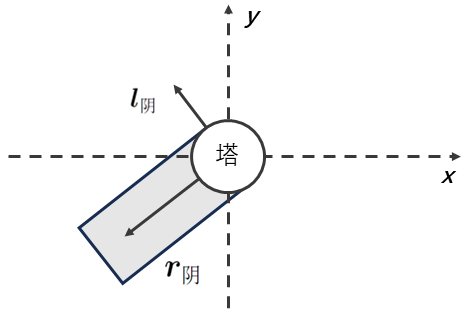
\includegraphics[width=2.6in]{问题1-1塔建系图.png}
		\caption{问题1塔$l-r$坐标系俯视图}
	\end{minipage}
	\begin{minipage}[b]{0.5\linewidth}
		\centering
		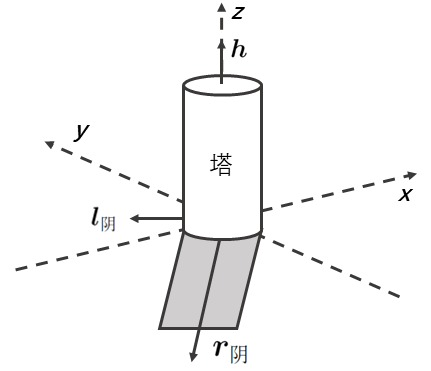
\includegraphics[width=2.4in]{问题1-1塔投影示意图.png}
		\caption{问题1塔$l-r-h$坐标系示意图}
	\end{minipage}
\end{figure}

\noindent
分析几何关系,易知方向向量$\bm{r_{\text{阴}}},\bm{l_{\text{阴}}}$仅与太阳方位角$\gamma_s$有关:
\begin{equation}
    \left\{\begin{array}{l}
        \bm{r_{\text{阴}}}=\left(-\sin \gamma_s,-\cos \gamma_s,0\right)\\
        \bm{l_{\text{阴}}}=\left(-\cos \gamma_s, \sin \gamma_s,0\right)\\
        \bm{h}=\left(0,0,1\right)
    \end{array}\right.
\end{equation}
若$0<\bm{p_{ij}}\cdot\bm{r_{\text{阴}}}\leq \frac{84}{\tan \alpha_s}$且$|\bm{p_{ij}}\cdot\bm{l_{\text{阴}}}|\leq\frac{7}{2}$
且$\frac{\bm{p_{ij}}\cdot\bm{h}}{\frac{84}{\tan \alpha_s}-\bm{p_{ij}}\cdot\bm{r_{\text{阴}}}}\leq \tan \alpha_s$,则点$\bm{p_{ij}}$在塔的阴影中。


\paragraph{(2-2)塔阴影遮挡判别器}
对每一时刻的$\bm{r_{\text{阴}}},\bm{l_{\text{阴}}},\bm{h}$,构建判别器判断$\bm{p_{ij}}$是否会被塔的阴影覆盖。
具体判别流程如下 (图12)
\begin{figure}[H]
    \centering
    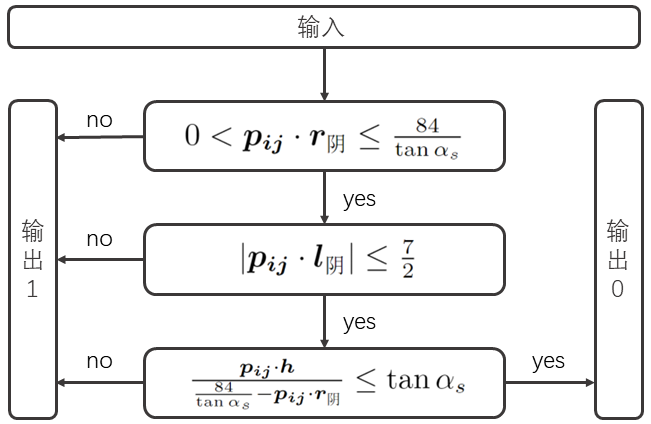
\includegraphics[scale=0.5]{问题1-1塔阴影遮挡判别器原理.png}
    \caption{问题1塔阴影遮挡判别器原理示意图}
\end{figure}

\paragraph{(3)综合判断结果}
将两个判断器的输出结果相乘得到综合判断结果,若为1则说明该点不会被阴影遮挡,若为0则说明该点会被遮挡。将一面镜子上所有点的综合判断结果相加并除以总点数,得到该定日镜的阴影遮挡效率$\eta_{sb}$(每面镜子上取点个数记为$M$):
\begin{equation}
    \eta_{sb}=\frac{1}{M}\sum_{j=1}^{M}\left(\text{定日镜阴影遮挡判别器输出}\right)\cdot\left(\text{塔阴影遮挡判别器输出}\right).
\end{equation}  

%--------------------------------------------------------------------
\subsubsection{集热器截断效率}

来自太阳的入射光线是一束锥形光线,其半角展宽为$4.65 mrad$\cite{3},根据反射原理,反射到吸热器上的光线
也是呈发散的锥形形状。目标点和反射镜的距离越远,光锥的截面越大。
由于镜场中定日镜到吸热塔的距离大小不一致,
吸热器上的反射光斑尺寸会根据定日镜与吸热器的距
离而有所变化。
此外,定日镜在制造过程中也存在一定的跟踪精度以
及面型精度。跟踪精度的存在会影响反射光斑是否精准地投射
到目标点上,而定日镜面型误差的存在会使反射光斑的形状不
再具有规则性。\cite{3}以上种种因素使镜场反射光斑并不能全部落
入吸热器接收范围内,而造成了一定的光溢出现象。故考虑集热器的截断效率$\eta_{trunc}$:

\begin{equation}
    \eta_{trunc}=\frac{\text{集热器接收能量}}{\text{镜面全反射能量 − 阴影遮挡损失能量}}.
\end{equation}

\vskip 0.25cm
由于反射光锥在集热器上的投影形状不规则,我们采用光线追迹法。
追迹一束太阳光中任意一条光线在经过定日镜反射后落入集热器的位置,
用集热器接受的光线数目除以反射光线的数目,即可得到集热器截断效率$\eta_{trunc}$。

\paragraph{(1)反射光线建模}

对于第$i$个定日镜上均匀取得的第$j$个点$\bm{p_{ij}}$(非阴影遮挡区域),反射光线呈锥形,半角展宽$\theta=4.65mrad$。
设反射光线方向向量$\bm{t_i}=(a_i,b_i,c_i)$,则可在镜场坐标系中找到另外两个方向向量$\bm{l_i},\bm{r_i}$,满足$\bm{l_i},\bm{r_i},\bm{t_i}$互相垂直(图13),即:%=================================================================

\begin{equation}
    \begin{aligned}
        &\bm{l_i}=\frac{1}{\sqrt{b_i^2+c_i^2}}\left(0,c_i,-b_i\right)\\
        &\bm{r_i}=\frac{1}{\sqrt{a_i^2b_i^2+a_i^2c_i^2+(b_i^2+c_i^2)^2}}\left(-b_i^2-c_i^2,a_i b_i,a_i c_i ,\right)\\
    \end{aligned}
\end{equation}

\vskip 0.25cm
\noindent
在第$i$个定日镜上第$j$个点的反射光锥中随机取光线。设取得的第$k$个光线的方向向量为$\bm{t_{ijk}}$,
$\bm{t_{ijk}}$与$\bm{t_s}$的夹角记为$\alpha$,$\bm{t_{ijk}}$在光锥切面圆上的投影与$\bm{l_i}$的夹角记为$\beta$。
令随机反射光线的取法满足$0\leq \alpha \leq\theta,0\leq \beta\leq 2\pi$的均匀分布(图14)。

\begin{figure}[htbp]
	\begin{minipage}[b]{0.5\linewidth}
		\centering
		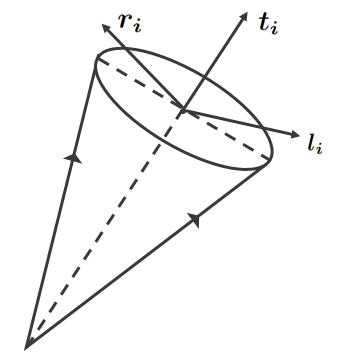
\includegraphics[width=1.55in]{问题1-1反射光锥建系图.png}
		\caption{问题1反射光锥$l-r-t$坐标系示意图}
	\end{minipage}
	\begin{minipage}[b]{0.5\linewidth}
		\centering
		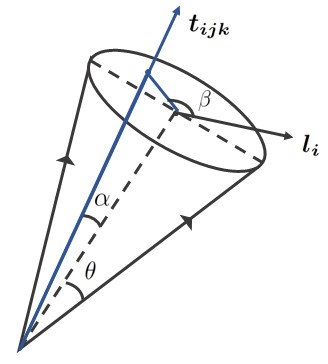
\includegraphics[width=1.5in]{问题1-1反射光锥随机光线示意图.png}
		\caption{问题1随机反射光线示意图}
	\end{minipage}
\end{figure}

\noindent
由几何关系可得,随机反射光线的方向向量$\bm{t_{ijk}}=\bm{t_i}+\tan\alpha\,(\cos\beta\,\bm{l_i}+\sin\beta\,\bm{r_i})$,

\noindent
则方向为$\bm{t_{ijk}}$的随机反射光线向量$\bm{\gamma_{ijk}}$可以参数化地表示为:$\bm{\gamma_{ijk}}=\bm{p_{ij}}+t\,\bm{t_{ijk}}$。

\paragraph{(2)光线追迹判别器}
对每一组$i,j,k$,构建判别器判断$\bm{\gamma_{ijk}}$与集热器曲面外侧是否有交点。
在镜场坐标系中,集热器的曲面方程为:
\begin{equation}
    \left\{\begin{array}{l}
        x^2+y^2=(\frac{7}{2})^2\\
        76\leq z\leq 84\\
    \end{array}\right.
\end{equation}

\noindent
记$\bm{\gamma_{ijk}}=(x,y,z),\bm{p_{ij}}=(x_{ij},y_{ij},z_{ij}),\bm{t_{ijk}}=(x_{ijk},y_{ijk},z_{ijk})$,由$\bm{\gamma_{ijk}}=\bm{p_{ij}}+t\,\bm{t_{ijk}}$可得:

\begin{equation}
    \left\{\begin{array}{l}
        x=x_{ij}+t\,x_{ijk}\\
        y=y_{ij}+t\,y_{ijk}\\
        z=z_{ij}+t\,z_{ijk}\\
    \end{array}\right.
\end{equation}

\noindent
其中$t$为参数。对于某一确定时刻,$x_{ij},y_{ij},z_{ij},x_{ijk},y_{ijk},z_{ijk}$均为确定常数。
由于(5.1.13)对$z$的范围有所限制,先仅考虑变量$x,y$。将(5.1.14)中$x,y$的表达式代入(5.1.13)中,得到关于参数$t$的一元二次方程:

\begin{equation}
        (x_{ij}+t\,x_{ijk})^2+(y_{ij}+t\,y_{ijk})^2=(\frac{7}{2})^2
\end{equation}

\vskip 0.25cm
\noindent
针对方程(5.1.15),构建判别流程如下(图15):
\begin{figure}[H]
    \centering
    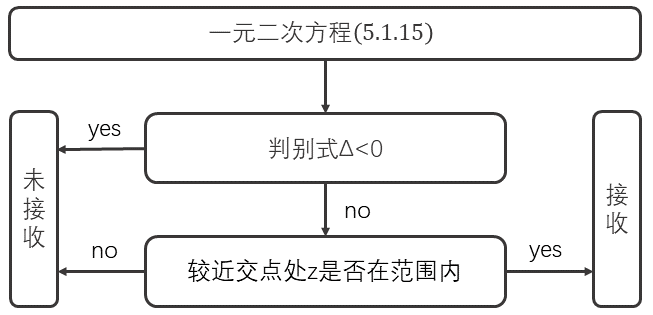
\includegraphics[scale=0.45]{问题1-1光线追踪判别器原理示意图.png}
    \caption{问题1光线追踪判别器原理示意图}
\end{figure}

\paragraph{(3)截断效率计算}
我们追迹了未被阴影遮挡处的随机反射光线落入集热器的位置,
用集热器接受的光线数目除以随机反射光线的总数目,即可得到集热器截断效率$\eta_{trunc}$。

\begin{equation}
    \eta_{trunc}=\frac{\text{集热器接收光线数目}}{\text{随机反射光线总数目}}.
\end{equation}
%--------------------------------------------------------------------
\subsubsection{余弦效率}
对于第$i$面定日镜,其入射光线与反射光线的方向向量分别记为$\bm{s_i},\bm{t_i}$,余弦效率$\eta_{\cos}$\cite{1}:
\begin{equation}
    \eta_{cos}=\bm{s_i}\cdot\bm{t_i}
\end{equation}

\subsubsection{光学效率}

设$d_{\mathrm{HR}}$表示镜面中心到集热器中心的距离,则:

大气透射率:$\eta_{\mathrm{at}}=0.99321-0.0001176 d_{\mathrm{HR}}+1.97 \times 10^{-8} \times d_{\mathrm{HR}}^2 \quad\left(d_{\mathrm{HR}} \leq 1000\right) $

定日镜的光学效率:$\eta=\eta_{\mathrm{sb}} \eta_{\mathrm{cos}} \eta_{\mathrm{at}} \eta_{\text {trunc}} \eta_{\mathrm{ref}}\quad\left(\eta_{\mathrm{ref}}=0.92\right) $

\subsubsection{输出热功率}
DNI (法向直接辐射辐照度) 是指地球上垂直于太阳光线的平面单位面积 上、单位时间内接收到的太阳辐射能量, 可按以下公式近似计算:
($G_0=1.366 \mathrm{~kW} / \mathrm{m}^2, H=3\mathrm{km}$)
\begin{equation}
    \left\{\begin{array}{l}
        \text {DNI}=G_0\left[a+b \exp \left(-\frac{c}{\sin \alpha_s}\right)\right] \\
        a=0.4237-0.00821(6-H)^2\\
        b=0.5055+0.00595(6.5-H)^2 \\
        c=0.2711+0.01858(2.5-H)^2\\
    \end{array}\right.
\end{equation}

\noindent
设$N$ 为定日镜总数,$A_i$ 为第 $i$ 面定日镜采光面积,$\eta_i$ 为第 $i$ 面镜子的光学效率,则定日镜场的输出热功率 $E_{\text {field }}$ 为:
\begin{equation}
    E_{\text {field }}=\mathrm{DNI} \cdot \sum_i^N A_i \eta_i,
\end{equation}

\subsection{问题一模型的求解}
定日镜共计1745面,每面镜子上均匀选取16个点,考虑周围5面镜子的阴影遮挡,$\alpha$在$[0,\theta]$区间内均匀选取4个值,$\beta$在$[0,2\pi]$区间内均匀选取8个值。
虽然理论上均匀采样数目越多得到的结果越精确,但现实受算力影响(程序运行时间7.5h)我们的设置采样数目较为保守。
对上述采样用python遍历输入模型(详见附录A),得到的结论数据如下表:
\begin{table}[!htbp]
    \centering
    \begin{tabular}{|c|c|c|c|c|c|}\hline
        日期&\makecell[c]{平均\\光学效率}&\makecell[c]{平均\\余弦效率}&\makecell[c]{平均阴影\\遮挡效率}&\makecell[c]{平均\\截断效率}&\makecell[c]{单位面积镜面平均输出\\热功率$(\mathrm{~kW} / \mathrm{m}^2)$}\\\hline
        1月21日&0.4705& 	0.7199& 	0.8905& 	0.8567& 0.4526         \\\hline
        2月21日&0.4838& 	0.7404& 	0.8865& 	0.8507& 0.4998         \\\hline
        3月21日&0.4876& 	0.7611& 	0.9040& 	0.8131& 0.5293         \\\hline
        4月21日&0.4995& 	0.7793& 	0.9045& 	0.8088& 0.5593         \\\hline
        5月21日&0.5041& 	0.7893& 	0.8982& 	0.8106& 0.5722         \\\hline
        6月21日&0.5046& 	0.7924& 	0.8934& 	0.8113& 0.5749         \\\hline
        7月21日&0.5041& 	0.7892& 	0.8983& 	0.8106& 0.5722         \\\hline
        8月21日&0.4984& 	0.7786& 	0.9035& 	0.8086& 0.5576         \\\hline
        9月21日&0.4869& 	0.7601& 	0.9038& 	0.8134& 0.5274         \\\hline
        10月21日&0.4720& 	0.7378& 	0.8969& 	0.8230& 0.4838         \\\hline
        11月21日&0.4608& 	0.7182& 	0.8994& 	0.8329& 0.4398  \\\hline
        12月21日&0.4522&	0.7111& 	0.8937&	0.8332& 0.4170  \\
        \hline
    \end{tabular}
    \caption{问题 1 每月 21 日平均光学效率及输出功率}
\end{table}

\begin{table}[!htbp]
    \centering
    \begin{tabular}{|c|c|c|c|c|c|}\hline
        \makecell[c]{年平均\\光学效率}&\makecell[c]{年平均\\余弦效率}&\makecell[c]{年平均阴影\\遮挡效率}&\makecell[c]{年平均\\截断效率}&\makecell[c]{年平均输出热\\功率$\mathrm{MW}$}&\makecell[c]{单位面积镜面年平均输出\\热功率$(\mathrm{~kW} / \mathrm{m}^2)$}\\\hline
        0.4854& 	0.7565& 	0.8977& 	0.8227&32.3843 &0.5155 
        \\\hline
    \end{tabular}
    \caption{问题 1 年平均光学效率及输出功率表}
\end{table}
%=================================================================


{\centering\section{问题二模型的建立与求解}}

\subsection{问题二模型的建立}
我们要在定日镜尺寸和安装高度相同的前提下,设计定日镜的尺寸、安装高度、数目,以及吸收塔与定日镜的位置坐标,使得定日镜场达到额定年平均输出功率$60MW$且单位镜面面积年平均输出热功率尽量大。
考虑到参数数目过多会导致运算量爆炸,我们采用了Campo布置方法\cite{7}对镜场模型参数进行简化,并采用PSO-GA算法对模型优化问题进行求解。

\subsubsection{初始镜场的Campo布置}
Campo是由FJ Collado等人\cite{7}提出的一种圆形定日镜场的布置方式。镜场由内到外分为不同的环形区域,同一区域内的定日镜尺寸、高度相同,各行上的定日镜数量也相同,从而可以大大减小定日镜场的参数维数(图16)。
首先从第一个布置区域的第一行开始排布,首行第一个定日镜放置在镜场的正北方向,其余定日镜以不发生机械碰撞为原则进行周向均匀布置。
第一行的半径$R_1(m)$由第一行的定日镜数量$Nhel_1$可通过计算得出:
\begin{equation}
    \left\{\begin{array}{l}
        R_1=(DM\cdot Nhel_1) / 2\pi\\
        DM=LW+desp\\
    \end{array}\right.
\end{equation}
其中$LW(m)$表示定日镜宽,$LH(m)$表示定日镜高,$DM(m)$为定日镜的特征圆直径,定日镜之间的安全距离$desp=5m$。
第二行定日镜数目与第一行相同,与第一行定日镜交错放置且使相邻行定日镜的特征圆相切,即相邻行的定日镜之间以最密方式排列(图17)。

\begin{figure}[htbp]
	\begin{minipage}[b]{0.5\linewidth}
		\centering
		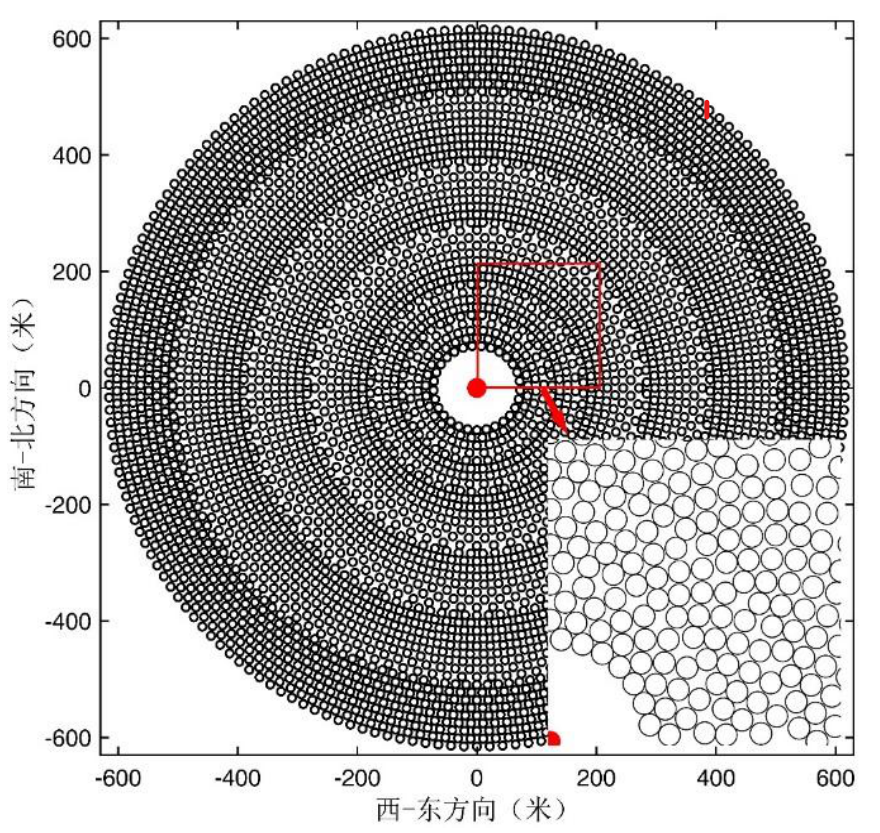
\includegraphics[width=2.5in]{问题2-1初始镜场示意图.png}
		\caption{问题2 Campo初始镜场排布方式示意图}
	\end{minipage}
	\begin{minipage}[b]{0.5\linewidth}
		\centering
		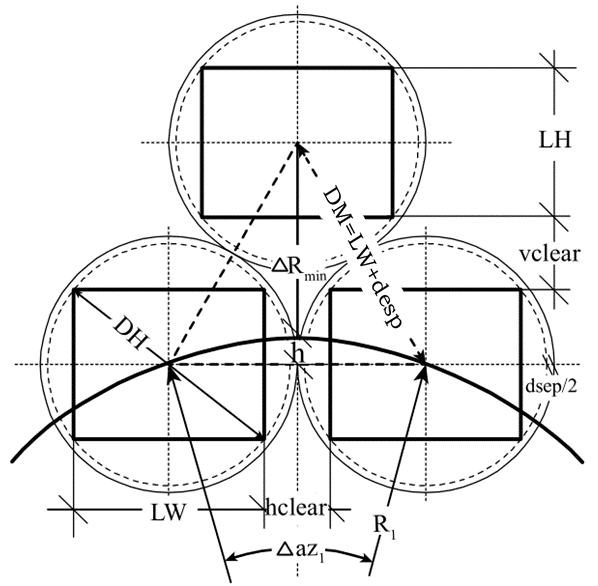
\includegraphics[width=2.5in]{问题2-1定日镜最密排列几何关系示意图.png}
		\caption{问题2定日镜最密集排布下的几何关系示意图}
	\end{minipage}
\end{figure}

由于在同一个区域各行定日镜的数量相同,所以奇数行与偶数行交错布置且连续行
之间的径向间距保持不变。在最密集的排布方式下,相邻行半径的最小增量$\Delta R_{min}$为:

\begin{equation}
    \left\{\begin{array}{l}
    \Delta R_{\min }=DM \cdot \cos 30^{\circ}-h \\
    h=R_1-\sqrt{R_1^2-\left({DM}^2 / 4\right)}
    \end{array}\right.
\end{equation}
\newpage
由于同一区域内各行上的定日镜数量保持不变,所以同一行上相邻定日镜之间的方
位间距会随着行半径的增加逐渐增大。当布置区域最后一行上两个相邻定日镜之间允许
放置一个额外的定日镜时,开始进行下一区域的布置,其排布原理同第一个区域相同。
因为下一区域内各行的定日镜数量为上一区域内各行定日镜数量的两倍,故各区域内每
行的定日镜数量$Nhel_n$与各区域首行的行半径$R_1^n$可由下式计算得出($n$为被布置区域的序号):
\begin{equation}
    \begin{aligned}
        &Nhel_n=Nhel_1 \cdot 2^{n-1}\\
        &R_n=R_1 \cdot 2^{n-1}\\
    \end{aligned}
\end{equation}
鉴于同一区域内相邻行之间的径向间距保持不变,可以根据这种特殊的布置关
系计算出第$n$区域内所能允许布置的最大行数$Nrows_n$
\begin{equation}
    {Nrows}_n=\frac{2^{n-1} \cdot R_1}{\Delta R_{\min }} \cong \operatorname{round}\left[\frac{2^{n-1} \cdot {DM} \cdot {Nhel}_1}{2 \pi\left({DM} \cdot \cos 30^{\circ}-h\right)}\right]
\end{equation}


\subsubsection{基于初始镜场的PSO-GA优化}

\paragraph{遗传算法(GA)}  
GA 是一种计算模型,选择、交叉和变异是其最常用的三种遗传操作。选择是从整个种群中挑选出几个适应度较高的个体来培育新
一代的过程。交叉是两个被选中的亲代个体交换部分基因以产生新个体的过程。突变会改变一个个体的一
个或多个基因值,这可以保持一代到下一代的遗传多样性,且 GA 群体可以通过突变操
作获得更好的解决方案。在选择之后,应用交叉和变异从这些被选中的个体中产生新的种群。

\paragraph{粒子群优化(PSO)}
PSO是一种基于种群的优化方法,其中每个粒子都会更新其位置和速度。
在每次迭代中,每个粒子都会通过跟踪自身之前的最佳位置(pbest)和群组之前的最佳位置
(gbest)来更新其速度和位置向量。
\begin{equation}
    \begin{aligned}
    & \mathrm{v}_{\mathrm{i}}(\mathrm{t}+1)=\mathrm{m} \cdot \mathrm{v}_{\mathrm{i}}(\mathrm{t})+\mathrm{c}_1 \mathrm{r}_1\left(\text {pbest}_{\mathrm{i}}(\mathrm{t})-\mathrm{x}_{\mathrm{i}}(\mathrm{t})\right)+\mathrm{c}_2 \mathrm{r}_2\left(\text {gbest}_{\mathrm{i}}(\mathrm{t})-\mathrm{x}_{\mathrm{i}}(\mathrm{t})\right) \\
    & x_i(t+1)=x_i(t)+v_i(t+1) \\
    & \mathrm{m}=\left\{\begin{array}{l}
    \mathrm{m}_{\min }+\frac{\left(\mathrm{m}_{\max }-\mathrm{m}_{\min }\right)\left(\mathrm{fit}-\mathrm{fit}_{\min }\right)}{\text {fit}_{\text {ave}}-\mathrm{fit}_{\min }}\leq \text {fit}_{\text {ave}} \\
    \mathrm{m}_{\max } \text {fit}>\mathrm{t}_{\text {ave}}
    \end{array}\right. \\
    \end{aligned}
\end{equation}

\paragraph{PSO-GA优化}
每种优化算法都有各自的优缺点。混合算法的思想能综合不同优化算法的优点,又能避免它们的缺点。\cite{8}
在PSO-GA算法中有七个参数$ m,c_1 ,c_2 ,r_1 ,r_2 ,Pc$ 和 $Pm$ 用于控制优化过程。$m$ 是自适应权重,用于根据上一代
种群中每个粒子的适合度控制算法的探索能力;
$c_1$ 和 $c_2$是两个加速度系数,均设置为 1.5。
$r_1$ 和 $r_2$ 是两个随机数,均匀分布在区间 $[0, 1]$ 内;
Pc 是 PSO-GA 中 GA 部分的交叉操作概率,设为 $0.8$;
Pm 是 PSO-GA 中 GA 部分的变异操作概率,设为 0.3。

\noindent
首先随机生成一个 PSO 群体,根据每个粒子的适应度确定 pbest 和 gbest。
继而根据每个粒子的位置和速度向量更新种群,执行交叉和突变操作并进一步更新种群中的粒子。
然后重新计算适应度,更新 pbest 和 gbest。最后检查停止标准,即当当前生成量达到最大
生成量(MG)或种群的适应度在 50 次迭代中保持不变。PSO-GA原理示意图如(图18)所示。

\begin{figure}[H]
    \centering
    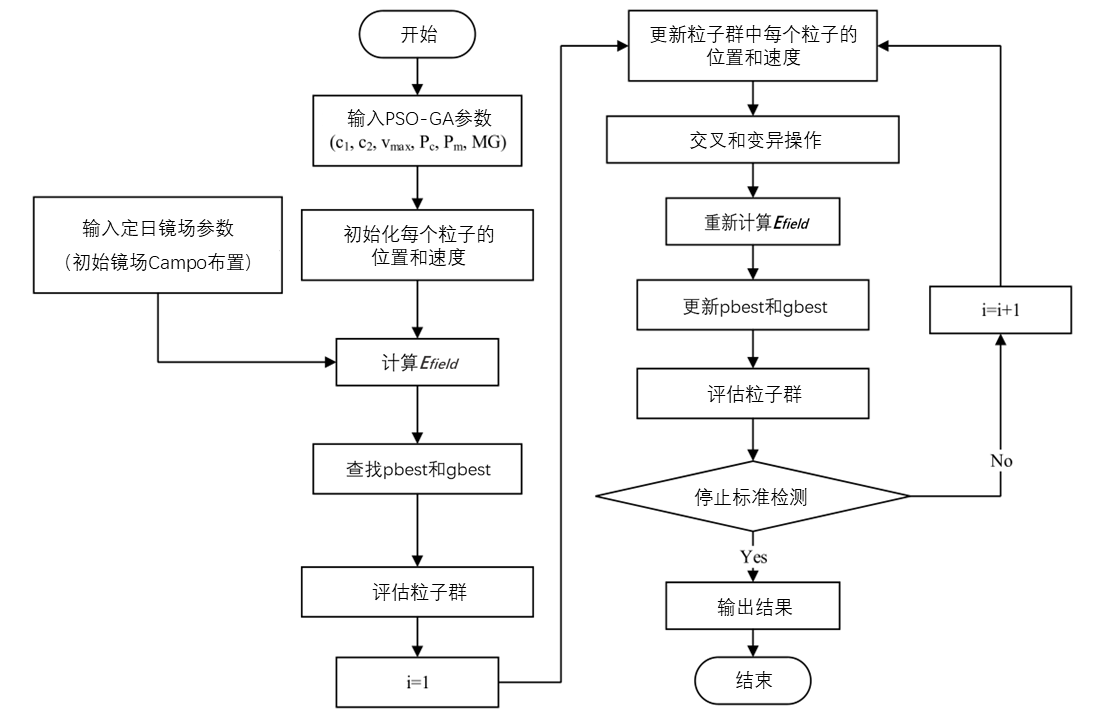
\includegraphics[scale=0.5]{问题2-1PSO-GA算法原理示意图.png}
    \caption{问题2 PSO-GA算法原理示意图}
\end{figure}

鉴于所有定日镜的尺寸和安装高度相同,初始Campo建模后我们仅需优化以下参数: 
\begin{table}[H]
    \centering
    \setlength{\tabcolsep}{12mm}{ %调整表格横向宽度
    \begin{tabular}{ccc}%调整表格列数
        \toprule[1.5pt]%调节横线1粗细
        符号 & 含义 & 维数\\
        \midrule[1pt]%调节横线2粗细
        $LH$&定日镜镜高 & 1\\
        $LW$&定日镜镜宽 & 1\\
        $h$&定日镜安装高度 & 1\\
        $r_i$&第$i$个区域第一行的半径&$i=4$\\
        $H_y$&集热塔的$y$轴坐标&1\\
        \bottomrule[1.5pt]%调节横线3粗细
    \end{tabular}}
    \caption{问题2模型优化参数列表}
\end{table}

\textbf{优化限制:}年平均输出热功率大于等于 $ 60 MW$,$100m\leq$镜与塔的距离$\leq 350m$。

\textbf{优化目标:}单位镜面面积年平均输出热功率尽量大。

\subsubsection{低效率镜点剔除}
初始镜场的Campo布置为圆环形,经过PSO-GA优化调参后整体布局仍为圆环形。
鉴于该镜场位于北半球北纬 39.4°,圆环形的镜场中极有可能存在低效率的镜点,拉低了镜场的单位镜面面积年平均输出热功率。
因此对于PSO-GA优化后的结果,需要设定合适的检验指标对各定日镜的年平均效率进行检测,将不达标的定日镜点提出,
使得定日镜场在达到额定功率的条件下单位镜
面面积年平均输出热功率尽量大。


\subsection{问题二模型的求解}


将上述定日镜场参数输入PSO-GA模型(详见附录B)得到优化后的参数数据。由于镜场单位面积平均输出热功率主要与定日镜的光学效率有关,所以计算优化后的定日镜的年平均光学效率作为剔除低效率镜点的依据。
按照光学效率从低到高的顺序分批剔除镜点,单位镜面面积年平均输出热功率逐渐增大,镜场的年平均输出功率逐渐减小,
直至镜场的年平均输出功率大于等于$60MW$,且继续剔除一个镜点会使镜场年平均输出功率小于$60MW$为止。
处理后得到镜场的优化分布如(图19)所示,定日镜的年平均功率以热图的形式呈现。

\begin{figure}[H]
    \centering
    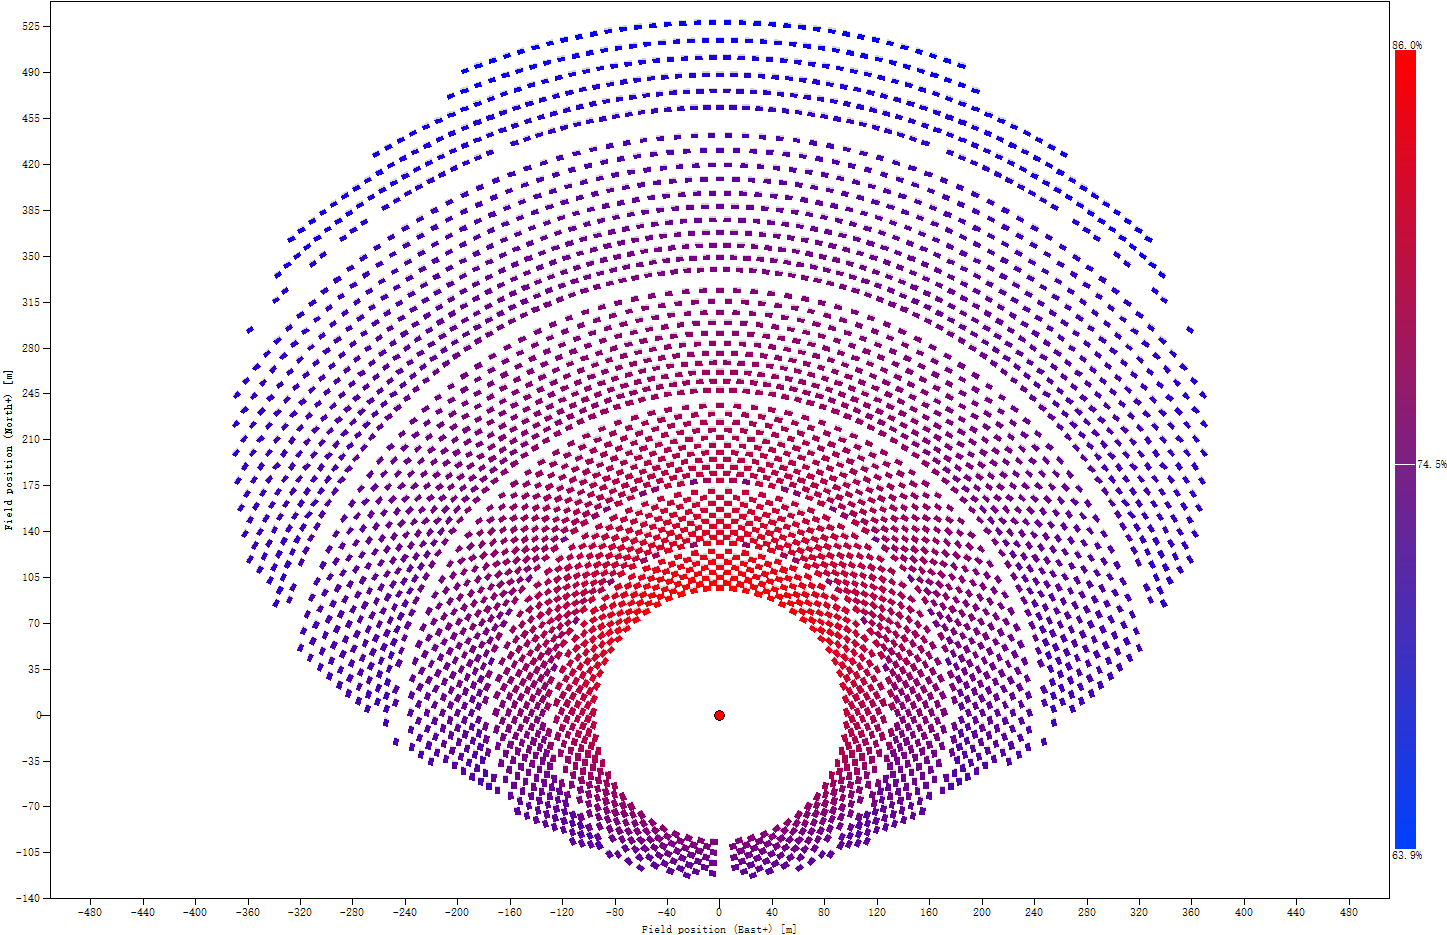
\includegraphics[scale=0.23]{问题2-2镜场优化分布功率热图.png}
    \caption{问题2镜场优化分布功率热图}
\end{figure}

将处理后的定日镜和集热塔坐标储存在附件result2.xlsx中,计算整理得结论数据如下表。




\begin{table}[!htbp]
    \centering
    \begin{tabular}{|c|c|c|c|c|c|}\hline
        日期&\makecell[c]{平均\\光学效率}&\makecell[c]{平均\\余弦效率}&\makecell[c]{平均阴影\\遮挡效率}&\makecell[c]{平均\\截断效率}&\makecell[c]{单位面积镜面平均输出\\热功率$(\mathrm{~kW} / \mathrm{m}^2)$}\\\hline
        1月21日&	0.7406& 	0.8812& 	0.9672& 	0.9845& 	0.7594 \\\hline
        2月21日&	0.7623& 	0.8808& 	0.9943& 	0.9856& 	0.7825 \\\hline
        3月21日&	0.7595& 	0.8746& 	0.9964& 	0.9867& 	0.8146 \\\hline
        4月21日&	0.7488& 	0.8609& 	0.9963& 	0.9880& 	0.8370 \\\hline
        5月21日&	0.7370& 	0.8466& 	0.9962& 	0.9888& 	0.8391 \\\hline
        6月21日&	0.7317& 	0.8402& 	0.9962& 	0.9891& 	0.8375 \\\hline
        7月21日&	0.7372& 	0.8468& 	0.9962& 	0.9888& 	0.8393 \\\hline
        8月21日&	0.7494& 	0.8617& 	0.9963& 	0.9879& 	0.8362 \\\hline
        9月21日&	0.7599& 	0.8751& 	0.9964& 	0.9867& 	0.8122 \\\hline
        10月21日&	0.7615& 	0.8811& 	0.9931& 	0.9855& 	0.7559 \\\hline
        11月21日&	0.7371& 	0.8811& 	0.9630& 	0.9844& 	0.6599 \\\hline
        12月21日&	0.7192& 	0.8787& 	0.9428& 	0.9839& 	0.7375 \\\hline
    \end{tabular}
    \caption{问题 2 每月 21 日平均光学效率及输出功率}
\end{table}

\begin{table}[!htbp]
    \centering
    \begin{tabular}{|c|c|c|c|c|c|}\hline
        \makecell[c]{年平均\\光学效率}&\makecell[c]{年平均\\余弦效率}&\makecell[c]{年平均阴影\\遮挡效率}&\makecell[c]{年平均\\截断效率}&\makecell[c]{年平均输出热\\功率$\mathrm{MW}$}&\makecell[c]{单位面积镜面年平均输出\\热功率$(\mathrm{~kW} / \mathrm{m}^2)$}\\\hline
        0.7453& 	0.8674& 	0.9862& 	0.9867& 	60.3426& 	0.7927
        \\\hline
    \end{tabular}
    \caption{问题 2 年平均光学效率及输出功率表}
\end{table}

\begin{table}[!htbp]
    \centering
    \begin{tabular}{|c|c|c|c|c|}\hline
        吸收塔位置坐标&\makecell[c]{定日镜尺寸\\(宽$\times$高)}&\makecell[c]{定日镜安装高度\\$(m)$}&定日镜总面数&\makecell[c]{定日镜总面积\\$(m^2)$}\\\hline
        (0,-210)&	5*4&	2.5&	3743&	74860
\\\hline
    \end{tabular}
    \caption{问题 2 设计参数表}
\end{table}
%=================================================================
{\centering\section{问题三模型的建立与求解}}

\subsection{问题三模型的建立}
问题三要求在定日镜尺寸及安装高度可以不同的条件下设计定日镜场的各个参数,使得镜场达
到额定年平均输出功率 $60MW$ 且单位镜面面积年平均输出热功率尽量大。
我们仍采用问题二中的Campo方法布置初始镜场,再用PSO-GA算法对模型优化问题进行求解,最后进行低效率镜点的剔除。
初始Campo建模后我们需要优化以下参数:

\begin{table}[H]
    \centering
    \setlength{\tabcolsep}{12mm}{ %调整表格横向宽度
    \begin{tabular}{ccc}%调整表格列数
        \toprule[1.5pt]%调节横线1粗细
        符号 & 含义 & 维数\\
        \midrule[1pt]%调节横线2粗细
        $LH_i$&第$i$个区域内定日镜镜高 & $i=4$\\
        $LW_i$&第$i$个区域内定日镜镜宽 & $i=4$\\
        $h_i$&第$i$个区域内定日镜安装高度 & $i=4$\\
        $r_i$&第$i$个区域第一行的半径&$i=4$\\
        $H_y$&集热塔的$y$轴坐标&1\\
        \bottomrule[1.5pt]%调节横线3粗细
    \end{tabular}}
    \caption{问题3模型优化参数列表}
\end{table}

\textbf{优化限制:}年平均输出热功率大于等于 $ 60 MW$,$100m\leq$镜与塔的距离$\leq 350m$。

\textbf{优化目标:}单位镜面面积年平均输出热功率尽量大。

\subsection{问题三模型的求解}

将上述定日镜场参数输入PSO-GA模型(详见附录C)得到优化后的参数数据。
按照光学效率从低到高的顺序分批剔除镜点,单位镜面面积年平均输出热功率逐渐增大,镜场的年平均输出功率逐渐减小,
直至镜场的年平均输出功率大于等于$60MW$,且继续剔除一个镜点会使镜场年平均输出功率小于$60MW$为止。
处理后得到镜场的优化分布如(图20)所示,定日镜的年平均功率以热图的形式呈现。

\begin{figure}[H]
    \centering
    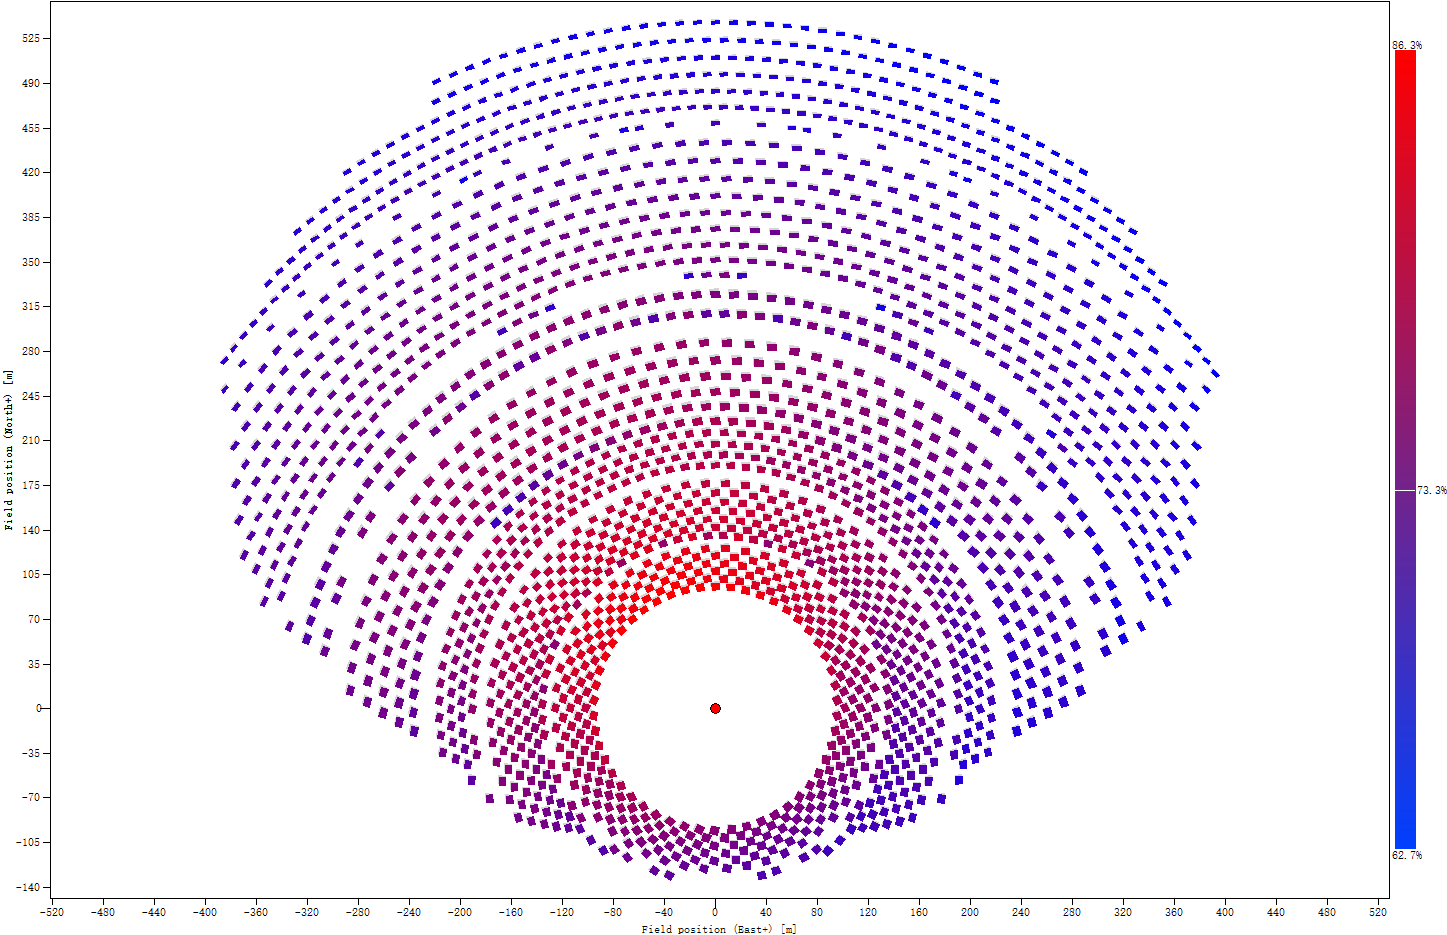
\includegraphics[scale=0.23]{问题3-2镜场优化分布功率热图.png}
    \caption{问题3镜场优化分布功率热图}
\end{figure}

将处理后的定日镜和集热塔尺寸及坐标储存在附件result3.xlsx中,整理得结论数据如下。

\begin{table}[!htbp]
    \centering
    \begin{tabular}{|c|c|c|c|c|c|}\hline
        日期&\makecell[c]{平均\\光学效率}&\makecell[c]{平均\\余弦效率}&\makecell[c]{平均阴影\\遮挡效率}&\makecell[c]{平均\\截断效率}&\makecell[c]{单位面积镜面平均输出\\热功率$(\mathrm{~kW} / \mathrm{m}^2)$}\\\hline
        1月21日&	0.7561& 	0.8799& 	0.9530& 	0.9758& 	0.7982\\\hline 
        2月21日&	0.7575& 	0.8793& 	0.9839& 	0.9776& 	0.8224 \\\hline 
        3月21日&	0.7537& 	0.8730& 	0.9922& 	0.9793 &	0.8561 \\\hline 
        4月21日&	0.7429& 	0.8588& 	0.9916 &	0.9810 &	0.8797 \\\hline 
        5月21日&	0.7312& 	0.8440& 	0.9913 &	0.9821 &	0.8818 \\\hline 
        6月21日&	0.7258& 	0.8374& 	0.9914 &	0.9825 &	0.8802 \\\hline 
        7月21日&	0.7313& 	0.8442& 	0.9913 &	0.9821 &	0.8820 \\\hline 
        8月21日&	0.7435& 	0.8596& 	0.9916 &	0.9809 &	0.8788 \\\hline 
        9月21日&	0.7541& 	0.8735& 	0.9922 &	0.9793 &	0.8536 \\\hline 
        10月21日&	0.7575& 	0.8796& 	0.9815 &	0.9774 &	0.7945 \\\hline 
        11月21日&	0.7559& 	0.8798 &	0.9487 &	0.9757 &	0.6935 \\\hline 
        12月21日&	0.7545& 	0.8792& 	0.9296 &	0.9749 &	0.7751 \\\hline 
    \end{tabular}
    \caption{问题 3 每月 21 日平均光学效率及输出功率}
\end{table}

\begin{table}[!htbp]
    \centering
    \begin{tabular}{|c|c|c|c|c|c|}\hline
        \makecell[c]{年平均\\光学效率}&\makecell[c]{年平均\\余弦效率}&\makecell[c]{年平均阴影\\遮挡效率}&\makecell[c]{年平均\\截断效率}&\makecell[c]{年平均输出热\\功率$\mathrm{MW}$}&\makecell[c]{单位面积镜面年平均输出\\热功率$(\mathrm{~kW} / \mathrm{m}^2)$}\\\hline
        0.7470& 	0.8657& 	0.9782& 	0.9791& 	61.4237& 	0.8331 
        \\\hline
    \end{tabular}
    \caption{问题 3 年平均光学效率及输出功率表}
\end{table}

\begin{table}[!htbp]
    \centering
    \begin{tabular}{|c|c|c|c|c|}\hline
        吸收塔位置坐标&\makecell[c]{定日镜尺寸\\(宽$\times$高)}&\makecell[c]{定日镜安装高度\\$(m)$}&定日镜总面数&\makecell[c]{定日镜总面积\\$(m^2)$}\\\hline
        (0,-200)&	-&	-&	2005&	73732
\\\hline
    \end{tabular}
    \caption{问题 3 年平均光学效率及输出功率表}
\end{table}
{\centering\section{模型的灵敏度分析}}
最后,为了检验光线追迹模型的稳定性,我们对问题1中结论数据进行了插值,插值曲面图与等高线图如下(图21)。
观察得到的“日期-时间-参量”曲面图可知:曲面的变化较为平缓,光线追迹的蒙特卡洛算法灵敏度较低,模型稳定性很好。 

\begin{figure}[!htbp]
	\centering
	\subfigure{
		\begin{minipage}[b]{0.42\textwidth}
			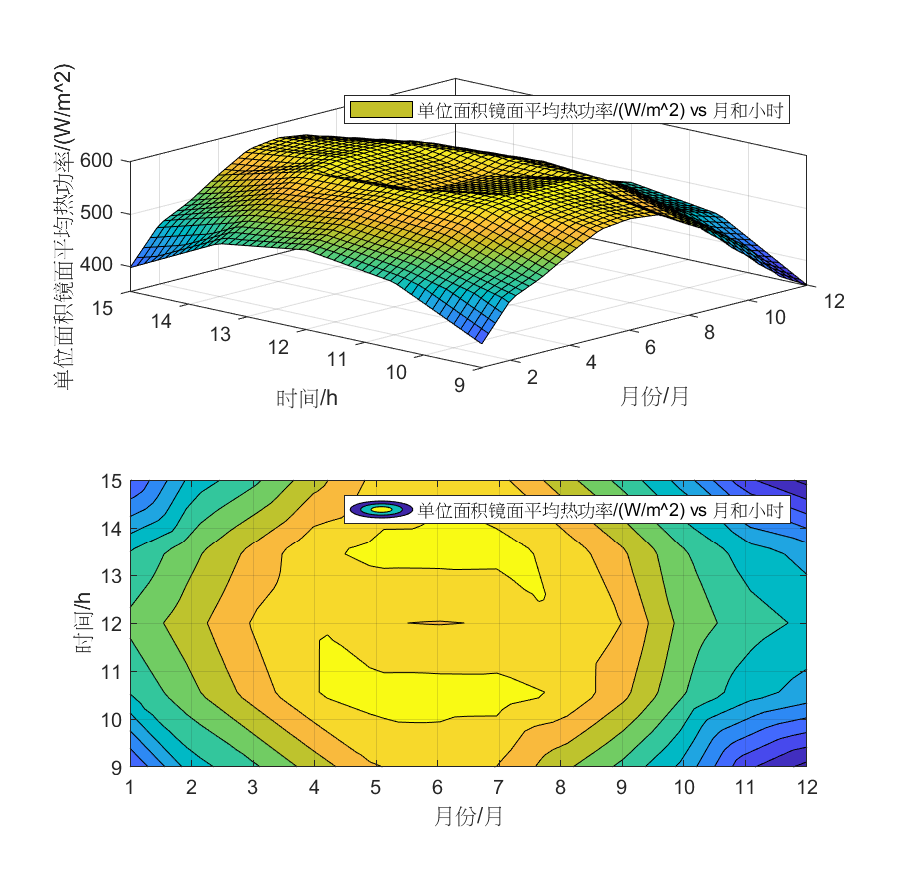
\includegraphics[width=1.2\textwidth]{eta.eps} 
		\end{minipage}
	}
    	\subfigure{
    		\begin{minipage}[b]{0.42\textwidth}
   		 	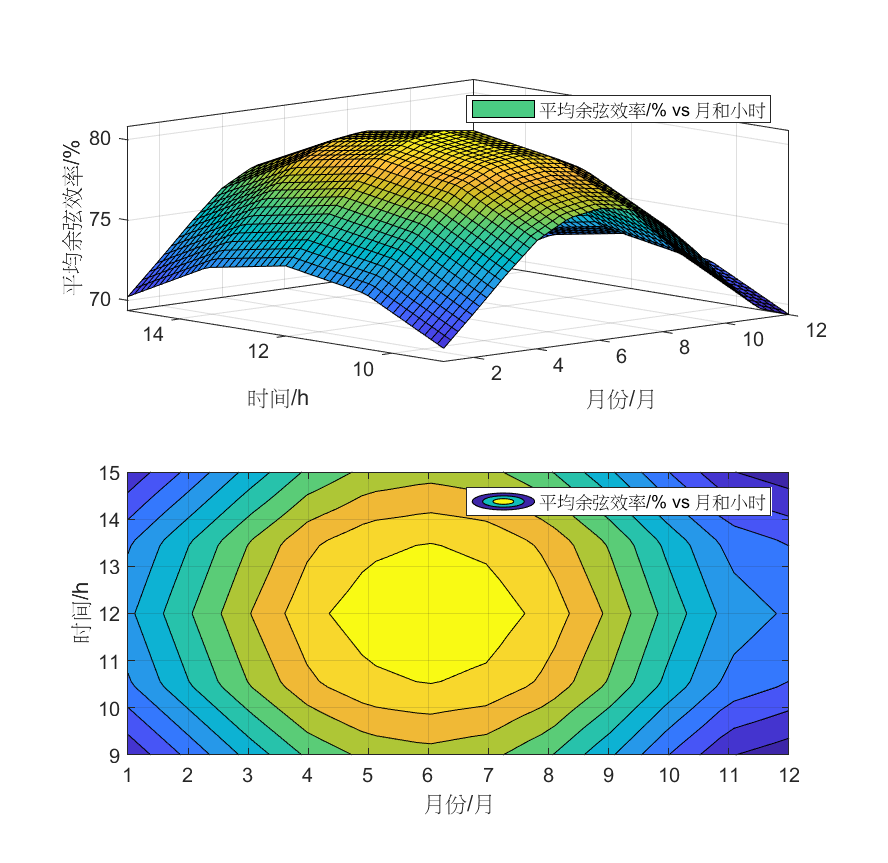
\includegraphics[width=1.2\textwidth]{eta_cos.eps}
    		\end{minipage}
    	}
	\\ 
	\subfigure{
		\begin{minipage}[b]{0.42\textwidth}
			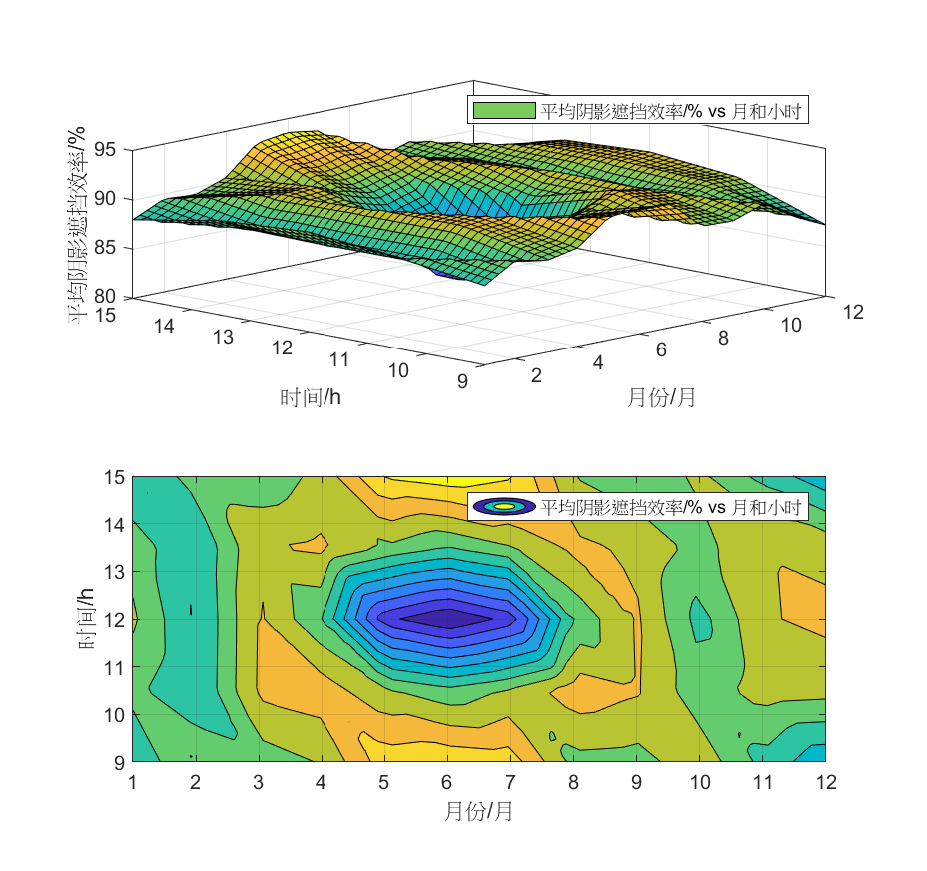
\includegraphics[width=1.2\textwidth]{eta_sb.eps} 
		\end{minipage}
	}
    	\subfigure{
    		\begin{minipage}[b]{0.42\textwidth}
		 	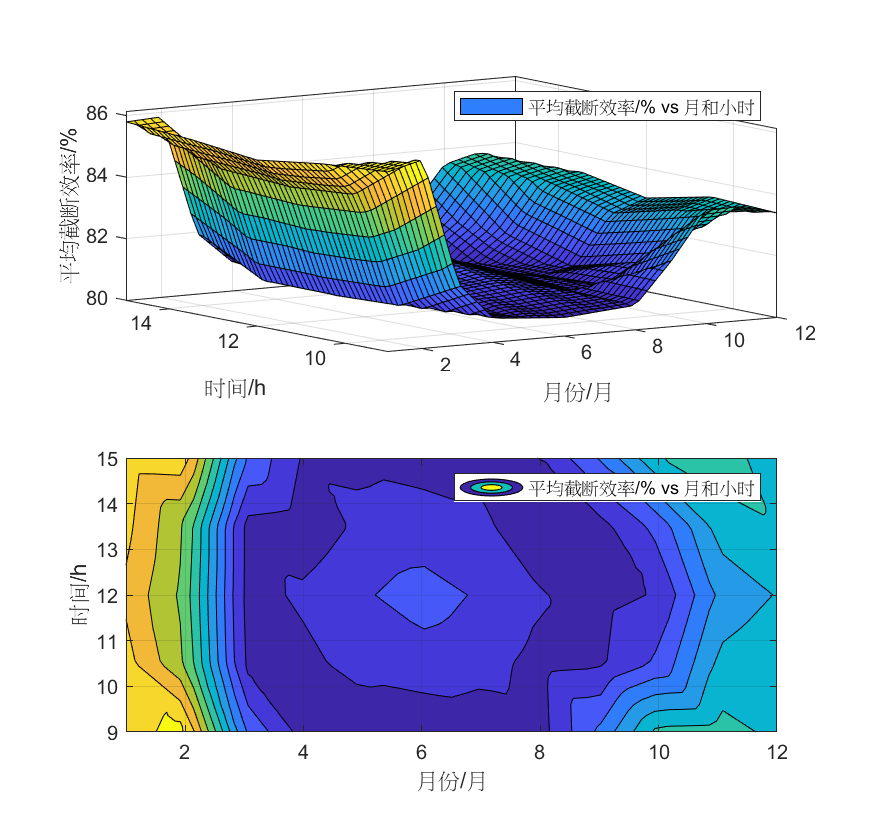
\includegraphics[width=1.2\textwidth]{eta_trunc.eps}
    		\end{minipage}
    	}
	\caption{问题1结论数据插值曲面图与等高线图}
\end{figure}


\newpage

{\centering\section{模型的评价与改进}}

\subsection{问题一模型的评价与改进}

\subparagraph{模型优点}~

1.周全考虑对阴影遮挡效率、截断效率造成损失的情况,建模直接,结论精确.

2.从统计意义上对截断效率,阴影遮挡效率采用均匀取点的蒙特卡洛法进行计算,单点误差服从正态分布,使得总体平均误差较小,可信度高。

\subparagraph{模型缺点}~

1.复杂度上计算时间较长。

2.阴影与遮挡效率的计算采用蒙特卡洛算法存在随机性,有一定的系统误差。

\subparagraph{模型改进}~

1.优化代码,用并行式计算减少计算时间。

2.若以计算精确度为优先,则可以考虑将截断模型的蒙特卡洛计算模拟改用太阳光能量分布的高斯模型进行改进。

3.若以降低时间计算复杂度为优先,考虑到截断效率平均都较高($>80\%$),可以考虑对截断效率以镜子关于塔的距离远近做分类,会极大减少计算量和时间。


\subsection{问题二、三模型的评价与改进}

\subparagraph{模型优点}~

1、利用Campo布置,很大程度减少变量数,大大降低计算量。

2、PSO-GA算法是群体智能算法,有利于在复杂函数内找到全局最优解。

3、截断效率用高斯分布近似,减少计算量。

\subparagraph{模型缺点}~

1、计算复杂度太大,耗时很久。

2、PSO-GA算法收敛速度慢,对初值敏感,不够稳定。

3、提前假设Campo布置为最佳布置方法,实际也有调整空间。

4、每个区域内所有定日镜的尺寸与高度可以不相等,固定为相等难以找到最优解。

5、高斯分布得到的截断效率与真实截断效率差距较大,并且没有考虑阴影遮挡,造成效率差距较大。

\subparagraph{模型改进}~

1、优化算法计算过程,加速计算速度。

2、适当细化变量,增加部分变量使得优化更加精确。

3、对真实截断效率进行曲线拟合,取得比高斯分布更加精确的结果。


{\centering\section{参考文献}}
\begingroup  % 去掉thebibliography环境自带的“参考文献”标题
\renewcommand{\section}[2]{}
\begin{thebibliography}{99}
    
\bibitem{1}
刘建兴. 塔式光热电站光学效率建模仿真及定日镜场优化布置[D].兰州: 兰州交通大学 , 2022.

\bibitem{2}
杜宇航, 刘向民, 王兴平, 蒋志浩. 塔式光热电站定日镜不同聚焦策略的影响分析[J] . 动力工程学报 , 2022.40(5) : 426-432

\bibitem{3}
张平,奚正稳,华文瀚,王娟娟,孙登科.太阳能塔式光热镜场光学效率计算方法[J] . 技术与市场 , 2021.28(6) : 5-8

\bibitem{4}
蔡志杰.太阳影子定位[J] . 数学建模及其应用 , 2015.4(4) : 25-33

\bibitem{5}
高博,刘建兴,孙浩,刘二林.基于自适应引力搜索算法的定日镜场优化布置[J] . 太阳能学报 , 2022.10(43) : 119-125

\bibitem{6}
O. Farges, J.J. Bezian, M. El Haf.Global optimization of solar power tower systems using a Monte Carlo algorithm Application to a redesign of the PS10 solar thermal power plant[J] . Renewable Energy, 2018 , 119 : 345-353

\bibitem{7}
Chao L, Zhai R, et al. Optimization of a heliostat field layout using hybrid PSO-GA algorithm[J].
Applied Thermal Engineering, 2018, 128(06):23-35

\bibitem{8}
Yu, S.; Zhang, J.; Zheng, S.; Sun, H. Provincial carbon intensity abatement potential estimation in China:
A PSO–GA-optimized multi-factor environmental learning curve method. Energy Policy2015, 77, 46–55.


\end{thebibliography}
\endgroup

\newpage



{\centering\section*{附录}}
\appendix
\section*{附件清单}
\begin{python}
    result2.xlsx
    result3.xlsx
    问题1代码实现
    问题2代码实现
    问题3代码实现
    论文编译
    参考文献
\end{python}    

\section{问题一代码实现}

确定太阳入射光线方向向量(\verb|sun_vector.py|)
\begin{python}
import datetime as datetime
import itertools
import pandas as pd
import numpy as np
import math


# 太阳时角计算
def get_omega(hour=9):
    omega = math.pi/12*(hour-12)
    return omega


def sun_vector(hour, phi=39.4, date='20220621', askfor='i') -> np.array:
    phi = phi*math.pi/180
    omega = get_omega(hour)     # 太阳时角

    cos_omega = math.cos(omega)
    sin_phi = math.sin(phi)
    cos_phi = math.cos(phi)
    date0 = datetime.date(2022,3,21)
    date = datetime.date(int(date[:4]),int(date[4:6]),int(date[6:]))
    D = (date-date0).days

    sin_delta = math.sin(2*math.pi*D/365)*math.sin(23.45*2*math.pi/360)  # 太阳赤纬角计算
    cos_delta = math.sqrt(1-sin_delta**2)

    sin_alpha_s = cos_delta*cos_phi*cos_omega + sin_delta * sin_phi
    cos_alpha_s = math.sqrt(1-sin_alpha_s**2)

    cos_gamma_s = round((sin_delta - sin_alpha_s*sin_phi)/(cos_alpha_s*cos_phi),5)
    if hour>12:
        sin_gamma_s = math.sqrt(1-cos_gamma_s**2)
    else:
        sin_gamma_s = -math.sqrt(1-cos_gamma_s**2)
    # 入射光线方向向量:
    if askfor=='i':
        i = np.array([cos_alpha_s*sin_gamma_s,cos_alpha_s*-cos_gamma_s,-sin_alpha_s])
        return i
    elif askfor=='sin_alpha_s':
        return sin_alpha_s
    elif askfor=='hlg':
        alpha_s = round(np.rad2deg(math.acos(cos_alpha_s)),2)
        if hour>12:
            gamma_s = round(360-np.rad2deg(math.acos(cos_gamma_s)),2)
        else:
            gamma_s = round(np.rad2deg(math.acos(cos_gamma_s)),2)
        return f'({alpha_s},{gamma_s})'
    elif askfor=='alpha_gamma_s':
        return sin_gamma_s,cos_gamma_s,sin_alpha_s/cos_alpha_s
    else:
        return None


def hlg_csv():
    hours = [9, 10.5, 12, 13.5, 15]
    dates = [f"2022{str(i).rjust(2, '0')}21" for i in range(1, 13)]
    df = pd.DataFrame(index=dates, columns=hours)
    for date, hour in itertools.product(dates, hours):
        df.loc[date, hour] = sun_vector(hour, phi=39.4, date=date, askfor='hlg')
    return df


if __name__ == '__main__':
    df = hlg_csv()
    df.to_csv('angle.csv')
\end{python}

确定镜子各个参数(\verb|class_mirror.py|)
\begin{python}
import numpy as np
import pandas as pd
from sun_vector import sun_vector



def normalize_vector(vector):
    return vector/np.linalg.norm(vector)


class mirror(object):
    tower_loc = np.array([0, 0, 80])

    def __init__(self, name, x, y, center_z=4, length=6, width=6):
        self.top5_list = None
        self.len2center = None
        self.eta_cos = None
        self.n = None
        self.light_area = None
        self.name = name
        self.x = x
        self.y = y
        self.center_z = center_z
        self.length = length
        self.width = width
        self.area = length * width
        # 镜子中心坐标
        self.mirror_loc = np.array([self.x, self.y, self.center_z])
        # 单位反射光线向量
        self.reflect_vec = normalize_vector(self.tower_loc - self.mirror_loc)
        # 计算大气透射率
        self.d_hr = np.linalg.norm(self.tower_loc - self.mirror_loc)

    # 镜面单位法向量
    def normal_vector(self, sun_vec):
        n = -sun_vec + self.reflect_vec
        n = n/np.linalg.norm(n)
        self.n = n
        return n

    def eta_cos(self, sun_vec):
        eta_cos = abs(sum(sun_vec * self.n))
        self.eta_cos = eta_cos
        return eta_cos

    def len2center(self,other):
        len2center = np.linalg.norm(self.mirror_loc - other.mirror_loc)
        return len2center
    
    def top5_close(self, mirror_list):
        for mirror_k in mirror_list:
            mirror_k.len2center = mirror.len2center(mirror_k, self)
        top5_list = sorted(mirror_list)[1:5]
        self.top5_list = top5_list
        return self

    def __lt__(self, other):
        return self.len2center < other.len2center
    # # 采光面积 用法向量和入射光线来算
    # def light_area(self, sun_vec, area=36):
    #     cos_theta = sum(sun_vec * self.n)
    #     self.light_area = area*cos_theta
    #     return area*cos_theta

def main():
    hour = 9
    sun_vec = sun_vector(hour, askfor='i')
    x, y = 150, -150
    mirror1 = mirror('mirror1', x, y)
    print('Successful Class')

if __name__ == '__main__':
    main()


\end{python}

计算阴影遮挡效率(\verb|eta_sb.py|)
\begin{python}
import itertools
import math
import time

import numpy as np
import pandas as pd
from sun_vector import sun_vector
from class_mirror import mirror
from eta_trunc import eta_trunc_1point


def normalize_vector(vector):
    return vector/np.linalg.norm(vector)

def eta_sb(mirror_i,sun_vec,r_shadow,l_shadow,tan_alpha_s,width=6,height=6):
    # start = time.time()
    alpha_list = np.linspace(0, 4.65e-3, 4)
    beta_list = np.linspace(0, 2 * np.pi, 8)
    mirror_i_loc = mirror_i.mirror_loc
    top5_list = mirror_i.top5_list       # exclude itself

    # 大柱子挡住 直接返回
    xij_r_shadow = np.dot(mirror_i_loc,r_shadow)
    if xij_r_shadow > 0 and xij_r_shadow <= 84 / tan_alpha_s and abs(np.dot(mirror_i_loc, l_shadow)) <= 3.5 and mirror_i_loc[2] / (
            84 / tan_alpha_s - xij_r_shadow) <= tan_alpha_s:
        return [0,0]

    ni = mirror_i.n; ni_x = ni[0];ni_y = ni[1];ni_z = ni[2]
    list_x = np.linspace(-width/2, width/2, 4)
    list_y = np.linspace(-height/2, height/2, 4)
    l_i = normalize_vector(np.array([ni_y, -ni_x, 0]))
    r_i = normalize_vector(np.array([-ni_x*ni_z, -ni_y*ni_z, ni_x**2+ni_y**2]))
    reflect_vec = mirror_i.reflect_vec
    count_df = pd.DataFrame({'eta_sb':[]})

    # print(round(end - start, 5), '最前面的一段s')

    # start_monte = time.time()
    for xij, yij in itertools.product(list_x,list_y):
        count_df.loc[f'({xij},{yij})','eta_sb'] = 0
        vec_xij = xij*l_i + yij*r_i + mirror_i_loc
        for mirror_k in top5_list:
            # start = time.time()
            mirror_k_n = mirror_k.n
            mirror_k_loc = mirror_k.mirror_loc
            nk_x = mirror_k_n[0]
            nk_y = mirror_k_n[1]
            nk_z = mirror_k_n[2]
            l_k = normalize_vector(np.array([nk_y, -nk_x, 0]))
            r_k = normalize_vector(np.array([-nk_x * nk_z, -nk_y * nk_z, nk_x ** 2 + nk_y ** 2]))
            aijk = vec_xij + np.dot(mirror_k_n,(mirror_k_loc-vec_xij))/np.dot(mirror_k_n, sun_vec)*sun_vec
            bijk = vec_xij + np.dot(mirror_k_n,(mirror_k_loc-vec_xij))/np.dot(mirror_k_n, reflect_vec)*reflect_vec
            # print(round(end - start, 5), '第一s')
            # start = time.time()
            if abs(np.dot((aijk - mirror_k_loc),l_k)) >= width/2:
                if abs(np.dot((aijk - mirror_k_loc),r_k)) >= height/2:
                    if abs(np.dot((bijk - mirror_k_loc),l_k)) >= width/2:
                        if abs(np.dot((bijk - mirror_k_loc) ,r_k)) >= height/2:
                            count_df.loc[f'({xij},{yij})','eta_sb'] = 1
                            count_df.loc[f'({xij},{yij})','eta_trunc_1point'] = eta_trunc_1point(reflect_vec,vec_xij,alpha_list,beta_list)
            # end = time.time()
            # print(round(end-start,5),'圆锥蒙特卡洛')
    # end_monte = time.time()
    # print(round(end_monte - start_monte, 5), '板蒙特卡洛 套蒙特卡洛s')

    # end = time.time()
    # print(round(end - start, 5), '一个点s')
    eta_sb = sum(count_df['eta_sb'])/len(count_df['eta_sb'])
    count_trunc = count_df[count_df['eta_sb'] == 1].copy()
    eta_trunc_whole = count_trunc['eta_trunc_1point'].mean()

    return [eta_sb,eta_trunc_whole]

# def get_nearst10_for():
#
def eta_at(d_hr):
    eta_at = 0.99321 - 0.0001176*d_hr + d_hr**2*1.97e-8
    return eta_at

# def eta_trunc(): # todo huge workload!!!!
#     return
#
# eta_ref = 0.92
# def eta()->pd.Series:
#     eta.name = 'eta'
#     return eta
\end{python}

计算集热器截断效率(\verb|eta_trunc.py|)
\begin{python}
import numpy as np
import pandas as pd
from sun_vector import sun_vector
import class_mirror as c_m
import itertools
import math
import time
from class_mirror import mirror

alpha = [0,2.325*10**(-4),4.65*10**(-3)]
beta = [0, 0.4*np.pi, 0.8*np.pi, 1.2*np.pi, 1.6*np.pi]

def normalize_vector(vector):
    return vector/np.linalg.norm(vector)

def cut_off(reflect_vec, chosen_x, alpha, beta):
    # reflect_vec = mirror.reflect_vec
    e_l = c_m.normalize_vector(np.array([0,reflect_vec[2], -reflect_vec[1]]))
    e_h = c_m.normalize_vector(np.array([-reflect_vec[2]**2-reflect_vec[1]**2, reflect_vec[0]*reflect_vec[1], reflect_vec[0]*reflect_vec[2]]))
    t_cut = reflect_vec + np.tan(alpha)*(np.cos(beta)*e_l + np.sin(beta)*e_h)
    a = t_cut[0]**2 + t_cut[1]**2
    b = 2*np.dot(t_cut[0:2],chosen_x[0:2])
    c = chosen_x[0]**2+chosen_x[1]**2-12.25
    sol = quadratic_solver(a,b,c)
    if sol == 'Error':
        return 0
    elif len(sol) == 1: #只有一个交点 相切
        if 76 <= chosen_x[2] + sol[0]*t_cut[2] <= 84:
            return 1
        else:
            return 0
    else:
        t = np.min(np.abs(sol))
        if 76 <= chosen_x[2] + t*t_cut[2] <= 84 :
            return 1
        else:
            return 0



def quadratic_solver(a,b,c):
    delta = b**2-4*a*c
    if delta < 0:
        return 'Error'
    elif delta == 0:
        return [-b/(2*a)]
    else:
        return [(-b + np.sqrt(delta))/(2*a), (-b - np.sqrt(delta))/(2*a)]

def eta_trunc_1point(reflect_vec,vec_xij,alpha_list,beta_list): # todo huge workload!!!!!
    count_series = pd.Series() # monte_carlo
    for alpha, beta in itertools.product(alpha_list,beta_list):
        count_series.loc[f'({alpha},{beta})'] = cut_off(reflect_vec, vec_xij, alpha, beta)
    eta_trunc_1point = sum(count_series)/len(count_series)
    return eta_trunc_1point

\end{python}

输出结论数据文件(\verb|q1_debug.py|)
\begin{python}
import math
import numpy as np
import pandas as pd
from sun_vector import sun_vector
from class_mirror import mirror, normalize_vector
import itertools
from eta_sb import *
import warnings
import time
warnings.filterwarnings('ignore')
from eta_sb import eta_sb


def dni(sin_alpha_s):
    g0 = 1366
    H = 3
    a = 0.4237 - 0.000821*((6-H)**2)
    b = 0.5055 + 0.00595*((6.5-H)**2)
    c = 0.2711 + 0.01858*((2.5-H)**2)
    dni = g0 * (a+b*math.exp(-c/sin_alpha_s))
    return dni


def main():
    hours = [9, 10.5, 12, 13.5, 15]
    dates = [f"2022{str(i).rjust(2,'0')}21" for i in range(3,5)]
    df = pd.read_csv(r'C:\Users\Administrator\Desktop\2023国赛\A题\Q1\mirror_loc.csv')
    df.columns = ['x', 'y']
    df['(x,y)'] = list(zip(df['x'],df['y'],df.index+1))
    df['id'] = df.index+1
    date_mean_table = pd.DataFrame({'hour': [], 'eta': [], 'eta_cos': [], 'eta_sb': [], 'eta_trunc': [], 'Efield': [], 'Efield_mirror_mean': []})
    hour_mean_table = {'hour': [], 'eta': [], 'eta_cos': [], 'eta_sb': [], 'eta_trunc': [], 'Efield': [],
                       'Efield_mirror_mean': []}

    df['mirrors'] = df['(x,y)'].apply(lambda x: mirror(x[2], x[0], x[1]))
    mirror_list = list(df['mirrors'])
    df['mirrors'] = df['mirrors'].apply(lambda x: mirror.top5_close(x, mirror_list))

    for date, hour in itertools.product(dates, hours):
        start = time.time()
        print('date',date)
        sun_vec = sun_vector(hour, phi=39.4, date=date)
        sin_alpha_s = sun_vector(hour, date=date, askfor='sin_alpha_s', phi=39.4)
        sin_gamma_s,cos_gamma_s,tan_alpha_s = sun_vector(hour, phi=39.4, date=date, askfor='alpha_gamma_s')
        r_shadow = np.array([-sin_gamma_s, -cos_gamma_s, 0])
        l_shadow = np.array([cos_gamma_s,-sin_gamma_s,0])

        df['normal_vec'] = df['mirrors'].apply(lambda x: mirror.normal_vector(x, sun_vec))
        df['eta_cos'] = df['mirrors'].apply(lambda x: mirror.eta_cos(x, sun_vec))
        df['eta_at'] = df['mirrors'].apply(lambda x: eta_at(x.d_hr))
        df['mirror_i_loc'] = df['mirrors'].apply(lambda x: x.mirror_loc)
        df['mirror_area'] = df['mirrors'].apply(lambda x: x.area)

        # todo big work!!!!!!!!!!!!!!
        df['eta_sb_trunc'] = df.apply(lambda x: eta_sb(x['mirrors'],sun_vec,r_shadow,l_shadow,tan_alpha_s,width=6,height=6),axis=1)            # todo get a series

        df['eta_sb'] = df['eta_sb_trunc'].apply(lambda x: x[0])
        df['eta_trunc'] = df['eta_sb_trunc'].apply(lambda x: x[1])
        df['eta'] = df['eta_sb']*df['eta_at']*df['eta_cos']*df['eta_trunc']*0.92
        E_field = dni(sin_alpha_s)*sum(df['mirror_area']*df['eta'])
        hour_mean_table['hour'].append(hour)
        hour_mean_table['eta'].append(df['eta'].mean())
        hour_mean_table['eta_cos'].append(df['eta_cos'].mean())
        hour_mean_table['eta_sb'].append(df['eta_sb'].mean())
        hour_mean_table['eta_trunc'].append(df['eta_trunc'].mean())
        hour_mean_table['Efield'].append(E_field)
        hour_mean_table['Efield_mirror_mean'].append(E_field/sum(df['mirror_area']))
        end = time.time()
        print('一天一个时辰',end-start,'s')
        insert_df = pd.DataFrame(hour_mean_table)
        insert_df.to_csv(f'{date}{hour}.csv')
        if len(hour_mean_table['hour']) == 5:
            hour_mean_map = pd.DataFrame(hour_mean_table)
            hour_mean_map.to_csv(f'{date}.csv')
            date_mean_table.loc[date] = hour_mean_map.mean()
            hour_mean_table = {'hour': [], 'eta': [], 'eta_cos': [], 'eta_sb': [], 'eta_trunc': [], 'Efield': [],
                       'Efield_mirror_mean': []}

    date_mean_table.to_csv('Q1.csv')
if __name__ == '__main__':
    main()
\end{python}

\section{问题二代码实现}

确定镜子各个参数(\verb|get_mirros_pos.py|)
\begin{python}
import pandas as pd

from class_mirror import mirror, normalize_vector
import itertools
from eta_sb import *
import warnings
import time

def get_mirrors_pos(r1,r2,r3,r4,c1,c2,c3,c4,
                       w1,w2,w3,w4,h1,h2,h3,h4,y_tower):
    # 定义参数
    tower_x = 0
    tower_y = y_tower
    tower_z = 0
    tower_radius = 100
    num_iterations = 6 #迭代次数
    mirrors_num = np.random.randint(5e6,6e6)
    df = pd.DataFrame({'x':np.random.random(mirrors_num),'y':np.random.random(mirrors_num)})

    # 定义六个半径和对应的尺寸
    radii = [r1]*4
    sizes = [c1, w1, h1]*4

    # 循环验证
    for iteration in range(1, num_iterations+1):
        test_df = perform_iteration(iteration,df,'20220321',hour=12)
    df = test_df

    # 生成均匀分布的点
    for radius, size in zip(radii, sizes):
        # 计算每个圆环上均匀分布的点数量,这里假设为100个
        num_points = 100

        # 生成均匀分布的角度
        angles = np.linspace(0, 2 * np.pi, num_points, endpoint=False)

        # 计算每个点的坐标
        x_coordinates = tower_x + radius * np.cos(angles)
        z_coordinates = tower_z + radius * np.sin(angles)

        # 创建一个DataFrame存储当前半径内的点
        radius_df = pd.DataFrame({'x': x_coordinates, 'y': tower_y, 'z': z_coordinates})

        # 添加尺寸信息
        radius_df['c'] = size[0]
        radius_df['w'] = size[1]
        radius_df['h'] = size[2]

        # 将当前半径内的点添加到总的DataFrame中
        df = df.append(radius_df, ignore_index=True)

    # 筛选出不在塔周围100米半径内的点
    distance_to_tower = np.sqrt((df['x'] - tower_x) ** 2 + (df['z'] - tower_z) ** 2)
    df = df[distance_to_tower > tower_radius]
    return df

def perform_iteration(iteration_number,df,date,hour):
    # 初始化参数
    df.columns = ['x', 'y']
    df['(x,y)'] = list(zip(df['x'],df['y'],df.index+1))
    df['id'] = df.index+1
    date_mean_table = pd.DataFrame({'hour': [], 'eta': [], 'eta_cos': [], 'eta_sb': [], 'eta_trunc': [], 'Efield': [], 'Efield_mirror_mean': []})
    hour_mean_table = {'hour': [], 'eta': [], 'eta_cos': [], 'eta_sb': [], 'eta_trunc': [], 'Efield': [],
                       'Efield_mirror_mean': []}

    df['mirrors'] = df['(x,y)'].apply(lambda x: mirror(x[2], x[0], x[1]))
    mirror_list = list(df['mirrors'])
    df['mirrors'] = df['mirrors'].apply(lambda x: mirror.top5_close(x, mirror_list))
    print('date',date)
    sun_vec = sun_vector(hour, phi=39.4, date=date)
    sin_alpha_s = sun_vector(hour, date=date, askfor='sin_alpha_s', phi=39.4)
    sin_gamma_s,cos_gamma_s,tan_alpha_s = sun_vector(hour, phi=39.4, date=date, askfor='alpha_gamma_s')
    r_shadow = np.array([-sin_gamma_s, -cos_gamma_s, 0])
    l_shadow = np.array([cos_gamma_s,-sin_gamma_s,0])
    df['eta_sb_trunc'] = df.apply(lambda x: eta_sb(x['mirrors'], sun_vec, r_shadow, l_shadow, tan_alpha_s, width=6, height=6), axis=1)
    return df


\end{python}

计算阴影遮挡效率(\verb|eta_sb.py|)
\begin{python}
import itertools
import math
import time

import numpy as np
import pandas as pd
from sun_vector import sun_vector
from class_mirror import mirror
from eta_trunc import eta_trunc_1point


def normalize_vector(vector):
    return vector/np.linalg.norm(vector)

def eta_sb(mirror_i,sun_vec,r_shadow,l_shadow,tan_alpha_s,width=6,height=6,center_z=4):
    alpha_list = np.linspace(0, 4.65e-3, 4)
    beta_list = np.linspace(0, 7/4 * np.pi, 8)
    mirror_i_loc = mirror_i.mirror_loc
    top5_list = mirror_i.top5_list       # exclude itself

    # 大柱子挡住 直接返回
    xij_r_shadow = np.dot(mirror_i_loc,r_shadow)
    if xij_r_shadow > 0 and xij_r_shadow <= 84 / tan_alpha_s and abs(np.dot(mirror_i_loc, l_shadow)) <= 3.5 and mirror_i_loc[2] / (
            84 / tan_alpha_s - xij_r_shadow) <= tan_alpha_s:
        return [0,0]

    ni = mirror_i.n; ni_x = ni[0];ni_y = ni[1];ni_z = ni[2]
    list_x = np.linspace(-width/2, width/2, 4)
    list_y = np.linspace(-height/2, height/2, 4)
    l_i = normalize_vector(np.array([ni_y, -ni_x, 0]))
    r_i = normalize_vector(np.array([-ni_x*ni_z, -ni_y*ni_z, ni_x**2+ni_y**2]))
    reflect_vec = mirror_i.reflect_vec
    count_df = pd.DataFrame({'eta_sb':[]})


    for xij, yij in itertools.product(list_x,list_y):
        count_df.loc[f'({xij},{yij})','eta_sb'] = 0
        vec_xij = xij*l_i + yij*r_i + mirror_i_loc
        for mirror_k in top5_list:
            mirror_k_n = mirror_k.n
            mirror_k_loc = mirror_k.mirror_loc
            nk_x = mirror_k_n[0]
            nk_y = mirror_k_n[1]
            nk_z = mirror_k_n[2]
            l_k = normalize_vector(np.array([nk_y, -nk_x, 0]))
            r_k = normalize_vector(np.array([-nk_x * nk_z, -nk_y * nk_z, nk_x ** 2 + nk_y ** 2]))
            aijk = vec_xij + np.dot(mirror_k_n,(mirror_k_loc-vec_xij))/np.dot(mirror_k_n, sun_vec)*sun_vec
            bijk = vec_xij + np.dot(mirror_k_n,(mirror_k_loc-vec_xij))/np.dot(mirror_k_n, reflect_vec)*reflect_vec

            if abs(np.dot((aijk - mirror_k_loc),l_k)) >= width/2:
                if abs(np.dot((aijk - mirror_k_loc),r_k)) >= height/2:
                    if abs(np.dot((bijk - mirror_k_loc),l_k)) >= width/2:
                        if abs(np.dot((bijk - mirror_k_loc) ,r_k)) >= height/2:
                            count_df.loc[f'({xij},{yij})','eta_sb'] = 1
                            count_df.loc[f'({xij},{yij})','eta_trunc_1point'] = eta_trunc_1point(reflect_vec,vec_xij,alpha_list,beta_list)


    eta_sb = sum(count_df['eta_sb'])/len(count_df['eta_sb'])
    count_trunc = count_df[count_df['eta_sb'] == 1].copy()
    eta_trunc_whole = count_trunc['eta_trunc_1point'].mean()

    return [eta_sb,eta_trunc_whole]


def eta_at(d_hr):
    eta_at = 0.99321 - 0.0001176*d_hr + d_hr**2*1.97e-8
    return eta_at


\end{python}

计算集热器截断效率(\verb|eta_trunc.py|)
\begin{python}
import numpy as np
import pandas as pd
from sun_vector import sun_vector
import class_mirror as c_m
import itertools
import math
import time
from class_mirror import mirror

alpha = [0,2.325*10**(-4),4.65*10**(-3)]
beta = [0, 0.4*np.pi, 0.8*np.pi, 1.2*np.pi, 1.6*np.pi]

def normalize_vector(vector):
    return vector/np.linalg.norm(vector)

def cut_off(reflect_vec, chosen_x, alpha, beta):
    # reflect_vec = mirror.reflect_vec
    e_l = c_m.normalize_vector(np.array([0,reflect_vec[2], -reflect_vec[1]]))
    e_h = c_m.normalize_vector(np.array([-reflect_vec[2]**2-reflect_vec[1]**2, reflect_vec[0]*reflect_vec[1], reflect_vec[0]*reflect_vec[2]]))
    t_cut = reflect_vec + np.tan(alpha)*(np.cos(beta)*e_l + np.sin(beta)*e_h)
    a = t_cut[0]**2 + t_cut[1]**2
    b = 2*np.dot(t_cut[0:2],chosen_x[0:2])
    c = chosen_x[0]**2+chosen_x[1]**2-12.25
    sol = quadratic_solver(a,b,c)
    if sol == 'Error':
        return 0
    elif len(sol) == 1: #只有一个交点 相切
        if 76 <= chosen_x[2] + sol[0]*t_cut[2] <= 84:
            return 1
        else:
            return 0
    else:
        t = np.min(np.abs(sol))
        if 76 <= chosen_x[2] + t*t_cut[2] <= 84 :
            return 1
        else:
            return 0



def quadratic_solver(a,b,c):
    delta = b**2-4*a*c
    if delta < 0:
        return 'Error'
    elif delta == 0:
        return [-b/(2*a)]
    else:
        return [(-b + np.sqrt(delta))/(2*a), (-b - np.sqrt(delta))/(2*a)]

def eta_trunc_1point(reflect_vec,vec_xij,alpha_list,beta_list): # todo huge workload!!!!!
    count_series = pd.Series() # monte_carlo
    for alpha, beta in itertools.product(alpha_list,beta_list):
        count_series.loc[f'({alpha},{beta})'] = cut_off(reflect_vec, vec_xij, alpha, beta)
    eta_trunc_1point = sum(count_series)/len(count_series)
    return eta_trunc_1point

\end{python}

PSO-GA算法(\verb|pso_ga_2.py|)
\begin{python}
import pandas as pd
from class_mirror import mirror, normalize_vector
import itertools
from eta_sb import *
import warnings
import time
from get_mirros_pos import get_mirrors_pos

def dni(sin_alpha_s):
    g0 = 1366
    H = 3
    a = 0.4237 - 0.000821*((6-H)**2)
    b = 0.5055 + 0.00595*((6.5-H)**2)
    c = 0.2711 + 0.01858*((2.5-H)**2)
    dni = g0 * (a+b*math.exp(-c/sin_alpha_s))
    return dni


# 定义适应度函数(目标函数)
def objective_function(r1, r2, r3, r4, c1,  c2, c3, c4,w1, w2, w3, w4, h1, h2, h3, h4 ,y_tower):
    hours = [9, 10.5, 12, 13.5, 15]
    dates = [f"2022{str(i).rjust(2,'0')}21" for i in range(3,5)]

    df_get_mirrors_pos = get_mirrors_pos(r1,r2,r3,r4,c1,c2,c3,c4,
                                w1,w2,w3,w4,h1,h2,h3,h4,y_tower)  # 得到每个镜子初始化坐标初始化
    df = df_get_mirrors_pos.copy()

    df.columns = ['x', 'y','c','w','h']
    df['(x,y)'] = list(zip(df['x'],df['y'],df.index+1))
    df['id'] = df.index+1
    date_mean_table = pd.DataFrame({'hour': [], 'eta': [], 'eta_cos': [], 'eta_sb': [], 'eta_trunc': [], 'Efield': [], 'Efield_mirror_mean': []})
    hour_mean_table = {'hour': [], 'eta': [], 'eta_cos': [], 'eta_sb': [], 'eta_trunc': [], 'Efield': [],
                       'Efield_mirror_mean': []}

    df['mirrors'] = df.apply(lambda x: mirror(x['(x,y)'][2], x['(x,y)'][0], x['(x,y)'][1],x['c'],x['w'],x['j']))
    mirror_list = list(df['mirrors'])
    df['mirrors'] = df['mirrors'].apply(lambda x: mirror.top5_close(x, mirror_list))
    E_field = []
    for date, hour in itertools.product(dates, hours):
        print('date',date)
        sun_vec = sun_vector(hour, phi=39.4, date=date)
        sin_alpha_s = sun_vector(hour, date=date, askfor='sin_alpha_s', phi=39.4)
        sin_gamma_s,cos_gamma_s,tan_alpha_s = sun_vector(hour, phi=39.4, date=date, askfor='alpha_gamma_s')
        r_shadow = np.array([-sin_gamma_s, -cos_gamma_s, 0])
        l_shadow = np.array([cos_gamma_s,-sin_gamma_s,0])

        df['normal_vec'] = df['mirrors'].apply(lambda x: mirror.normal_vector(x, sun_vec))
        df['eta_cos'] = df['mirrors'].apply(lambda x: mirror.eta_cos(x, sun_vec))
        df['eta_at'] = df['mirrors'].apply(lambda x: eta_at(x.d_hr))
        df['mirror_i_loc'] = df['mirrors'].apply(lambda x: x.mirror_loc)
        df['mirror_area'] = df['mirrors'].apply(lambda x: x.area)

        df['eta_sb_trunc'] = df.apply(lambda x: eta_sb(x['mirrors'], sun_vec, r_shadow, l_shadow, tan_alpha_s, width=x['w'], height=x['h'], center_z=x['c']),axis=1)            # todo get a series

        df['eta_sb'] = df['eta_sb_trunc'].apply(lambda x: x[0])
        df['eta_trunc'] = df['eta_sb_trunc'].apply(lambda x: x[1])
        df['eta'] = df['eta_sb']*df['eta_at']*df['eta_cos']*df['eta_trunc']*0.92
        E_field.append(dni(sin_alpha_s)*sum(df['mirror_area']*df['eta']))
    E_field_mean = pd.Series(E_field).mean()
    return E_field_mean


# PSO-GA算法
def pso_ga(objective_function, num_particles, num_dimensions, max_iterations,
           m, c1, c2, Pc, Pm):
    # 初始化粒子群和GA种群
    swarm_position = np.random.rand(num_particles, num_dimensions)
    swarm_velocity = np.random.rand(num_particles, num_dimensions)
    ga_population = np.random.rand(num_particles, num_dimensions)


    best_swarm_position = swarm_position.copy()
    best_swarm_value = np.zeros(num_particles)

    for i in range(num_particles):
        r1, c1, w1, h1, y_tower = list(swarm_position[i])
        r1, r2, r3, r4 = [r1] * 4
        c1, c2, c3, c4 = [c1] * 4
        w1, w2, w3, w4 = [w1] * 4
        h1, h2, h3, h4 = [h1] * 4
        best_swarm_value[i] = objective_function(r1, r2, r3, r4,  c1, c2, c3, c4,w1, w2, w3, w4, h1, h2, h3, h4, y_tower)

    global_best_index = np.argmin(best_swarm_value)
    global_best_position = swarm_position[global_best_index]
    global_best_value = best_swarm_value[global_best_index]

    for iteration in range(max_iterations):
        for i in range(num_particles):
            current_value = objective_function(swarm_position[i])

            if current_value < best_swarm_value[i]:
                best_swarm_position[i] = swarm_position[i]
                best_swarm_value[i] = current_value

            if current_value < global_best_value:
                global_best_position = swarm_position[i]
                global_best_value = current_value

            r1, r2 = np.random.rand(), np.random.rand()
            swarm_velocity[i] = (m * swarm_velocity[i] +
                                  c1 * r1 * (best_swarm_position[i] - swarm_position[i]) +
                                  c2 * r2 * (global_best_position - swarm_position[i]))
            swarm_position[i] += swarm_velocity[i]

        selected_parents = np.random.choice(num_particles, num_particles // 2, replace=True)
        offspring = []
        for i in range(0, num_particles, 2):
            parent1, parent2 = selected_parents[i], selected_parents[i + 1]
            crossover_point = np.random.randint(num_dimensions)
            child1 = np.concatenate((ga_population[parent1][:crossover_point], ga_population[parent2][crossover_point:]))
            child2 = np.concatenate((ga_population[parent2][:crossover_point], ga_population[parent1][crossover_point:]))
            offspring.extend([child1, child2])

        offspring = np.array(offspring)

        crossover_mask = np.random.rand(num_particles, num_dimensions) < Pc
        ga_population[crossover_mask] = offspring[crossover_mask]

        mutation_mask = np.random.rand(num_particles, num_dimensions) < Pm
        mutation_values = np.random.rand(num_particles, num_dimensions)
        ga_population[mutation_mask] = mutation_values[mutation_mask]
    return global_best_position, global_best_value


def main():
    num_particles = 20
    num_dimensions = 5
    max_iterations = 100
    m = 0.5
    c1 = 1.5
    c2 = 1.5
    Pc = 0.8
    Pm = 0.3

    best_position, best_value = pso_ga(objective_function, num_particles, num_dimensions, max_iterations,
                                       m, c1, c2, Pc, Pm)
    series = pd.Series(best_position,best_position)
    series.to_csv('result.csv')
if __name__ == '__main__':
    main()
\end{python}

\section{问题三代码实现}

确定镜子各个参数(\verb|get_mirros_pos.py|)
\begin{python}
import pandas as pd

from class_mirror import mirror, normalize_vector
import itertools
from eta_sb import *
import warnings
import time

def get_mirrors_pos(r1,r2,r3,r4,c1,c2,c3,c4,
                       w1,w2,w3,w4,h1,h2,h3,h4,y_tower):
    # 定义参数
    tower_x = 0
    tower_y = y_tower
    tower_z = 0
    tower_radius = 100
    num_iterations = 6 #迭代次数
    mirrors_num = np.random.randint(5e5,6e5)
    df = pd.DataFrame({'x':np.random.random(mirrors_num),'y':np.random.random(mirrors_num)})

    # 定义六个半径和对应的尺寸
    radii = [r1, r2, r3, r4,]
    sizes = [c1, w1, h1, c2, w2, h2, c3, w3, h3, c4, w4, h4]

    # 循环验证
    for iteration in range(1, num_iterations+1):
        test_df = perform_iteration(iteration,df,'20220321',hour=12)
    df = test_df

    # 生成均匀分布的点
    for radius, size in zip(radii, sizes):
        # 计算每个圆环上均匀分布的点数量,这里假设为100个
        num_points = 100

        # 生成均匀分布的角度
        angles = np.linspace(0, 2 * np.pi, num_points, endpoint=False)

        # 计算每个点的坐标
        x_coordinates = tower_x + radius * np.cos(angles)
        z_coordinates = tower_z + radius * np.sin(angles)

        # 创建一个DataFrame存储当前半径内的点
        radius_df = pd.DataFrame({'x': x_coordinates, 'y': tower_y, 'z': z_coordinates})

        # 添加尺寸信息
        radius_df['c'] = size[0]
        radius_df['w'] = size[1]
        radius_df['h'] = size[2]

        # 将当前半径内的点添加到总的DataFrame中
        df = df.append(radius_df, ignore_index=True)

    # 筛选出不在塔周围100米半径内的点
    distance_to_tower = np.sqrt((df['x'] - tower_x) ** 2 + (df['z'] - tower_z) ** 2)
    df = df[distance_to_tower > tower_radius]
    return df

def perform_iteration(iteration_number,df,date,hour):
    # 初始化参数
    df.columns = ['x', 'y']
    df['(x,y)'] = list(zip(df['x'],df['y'],df.index+1))
    df['id'] = df.index+1
    date_mean_table = pd.DataFrame({'hour': [], 'eta': [], 'eta_cos': [], 'eta_sb': [], 'eta_trunc': [], 'Efield': [], 'Efield_mirror_mean': []})
    hour_mean_table = {'hour': [], 'eta': [], 'eta_cos': [], 'eta_sb': [], 'eta_trunc': [], 'Efield': [],
                       'Efield_mirror_mean': []}

    df['mirrors'] = df['(x,y)'].apply(lambda x: mirror(x[2], x[0], x[1]))
    mirror_list = list(df['mirrors'])
    df['mirrors'] = df['mirrors'].swifter.apply(lambda x: mirror.top5_close(x, mirror_list))
    print('date',date)
    sun_vec = sun_vector(hour, phi=39.4, date=date)
    sin_alpha_s = sun_vector(hour, date=date, askfor='sin_alpha_s', phi=39.4)
    sin_gamma_s,cos_gamma_s,tan_alpha_s = sun_vector(hour, phi=39.4, date=date, askfor='alpha_gamma_s')
    r_shadow = np.array([-sin_gamma_s, -cos_gamma_s, 0])
    l_shadow = np.array([cos_gamma_s,-sin_gamma_s,0])
    df['eta_sb_trunc'] = df.apply(lambda x: eta_sb(x['mirrors'], sun_vec, r_shadow, l_shadow, tan_alpha_s, width=6, height=6), axis=1)
    return df


\end{python}

计算阴影遮挡效率(\verb|eta_sb.py|)
\begin{python}
import itertools
import math
import time

import numpy as np
import pandas as pd
from sun_vector import sun_vector
from class_mirror import mirror
from eta_trunc import eta_trunc_1point


def normalize_vector(vector):
    return vector/np.linalg.norm(vector)

def eta_sb(mirror_i,sun_vec,r_shadow,l_shadow,tan_alpha_s,width=6,height=6,center_z=4):
    alpha_list = np.linspace(0, 4.65e-3, 4)
    beta_list = np.linspace(0, 7/4 * np.pi, 8)
    mirror_i_loc = mirror_i.mirror_loc
    top5_list = mirror_i.top5_list       # exclude itself

    # 大柱子挡住 直接返回
    xij_r_shadow = np.dot(mirror_i_loc,r_shadow)
    if xij_r_shadow > 0 and xij_r_shadow <= 84 / tan_alpha_s and abs(np.dot(mirror_i_loc, l_shadow)) <= 3.5 and mirror_i_loc[2] / (
            84 / tan_alpha_s - xij_r_shadow) <= tan_alpha_s:
        return [0,0]

    ni = mirror_i.n; ni_x = ni[0];ni_y = ni[1];ni_z = ni[2]
    list_x = np.linspace(-width/2, width/2, 4)
    list_y = np.linspace(-height/2, height/2, 4)
    l_i = normalize_vector(np.array([ni_y, -ni_x, 0]))
    r_i = normalize_vector(np.array([-ni_x*ni_z, -ni_y*ni_z, ni_x**2+ni_y**2]))
    reflect_vec = mirror_i.reflect_vec
    count_df = pd.DataFrame({'eta_sb':[]})


    for xij, yij in itertools.product(list_x,list_y):
        count_df.loc[f'({xij},{yij})','eta_sb'] = 0
        vec_xij = xij*l_i + yij*r_i + mirror_i_loc
        for mirror_k in top5_list:
            mirror_k_n = mirror_k.n
            mirror_k_loc = mirror_k.mirror_loc
            nk_x = mirror_k_n[0]
            nk_y = mirror_k_n[1]
            nk_z = mirror_k_n[2]
            l_k = normalize_vector(np.array([nk_y, -nk_x, 0]))
            r_k = normalize_vector(np.array([-nk_x * nk_z, -nk_y * nk_z, nk_x ** 2 + nk_y ** 2]))
            aijk = vec_xij + np.dot(mirror_k_n,(mirror_k_loc-vec_xij))/np.dot(mirror_k_n, sun_vec)*sun_vec
            bijk = vec_xij + np.dot(mirror_k_n,(mirror_k_loc-vec_xij))/np.dot(mirror_k_n, reflect_vec)*reflect_vec

            if abs(np.dot((aijk - mirror_k_loc),l_k)) >= width/2:
                if abs(np.dot((aijk - mirror_k_loc),r_k)) >= height/2:
                    if abs(np.dot((bijk - mirror_k_loc),l_k)) >= width/2:
                        if abs(np.dot((bijk - mirror_k_loc) ,r_k)) >= height/2:
                            count_df.loc[f'({xij},{yij})','eta_sb'] = 1
                            count_df.loc[f'({xij},{yij})','eta_trunc_1point'] = eta_trunc_1point(reflect_vec,vec_xij,alpha_list,beta_list)


    eta_sb = sum(count_df['eta_sb'])/len(count_df['eta_sb'])
    count_trunc = count_df[count_df['eta_sb'] == 1].copy()
    eta_trunc_whole = count_trunc['eta_trunc_1point'].mean()

    return [eta_sb,eta_trunc_whole]


def eta_at(d_hr):
    eta_at = 0.99321 - 0.0001176*d_hr + d_hr**2*1.97e-8
    return eta_at


\end{python}

计算集热器截断效率(\verb|eta_trunc.py|)
\begin{python}
import numpy as np
import pandas as pd
from sun_vector import sun_vector
import class_mirror as c_m
import itertools
import math
import time
from class_mirror import mirror

alpha = [0,2.325*10**(-4),4.65*10**(-3)]
beta = [0, 0.4*np.pi, 0.8*np.pi, 1.2*np.pi, 1.6*np.pi]

def normalize_vector(vector):
    return vector/np.linalg.norm(vector)

def cut_off(reflect_vec, chosen_x, alpha, beta):
    # reflect_vec = mirror.reflect_vec
    e_l = c_m.normalize_vector(np.array([0,reflect_vec[2], -reflect_vec[1]]))
    e_h = c_m.normalize_vector(np.array([-reflect_vec[2]**2-reflect_vec[1]**2, reflect_vec[0]*reflect_vec[1], reflect_vec[0]*reflect_vec[2]]))
    t_cut = reflect_vec + np.tan(alpha)*(np.cos(beta)*e_l + np.sin(beta)*e_h)
    a = t_cut[0]**2 + t_cut[1]**2
    b = 2*np.dot(t_cut[0:2],chosen_x[0:2])
    c = chosen_x[0]**2+chosen_x[1]**2-12.25
    sol = quadratic_solver(a,b,c)
    if sol == 'Error':
        return 0
    elif len(sol) == 1: #只有一个交点 相切
        if 76 <= chosen_x[2] + sol[0]*t_cut[2] <= 84:
            return 1
        else:
            return 0
    else:
        t = np.min(np.abs(sol))
        if 76 <= chosen_x[2] + t*t_cut[2] <= 84 :
            return 1
        else:
            return 0



def quadratic_solver(a,b,c):
    delta = b**2-4*a*c
    if delta < 0:
        return 'Error'
    elif delta == 0:
        return [-b/(2*a)]
    else:
        return [(-b + np.sqrt(delta))/(2*a), (-b - np.sqrt(delta))/(2*a)]

def eta_trunc_1point(reflect_vec,vec_xij,alpha_list,beta_list): # todo huge workload!!!!!
    count_series = pd.Series() # monte_carlo
    for alpha, beta in itertools.product(alpha_list,beta_list):
        count_series.loc[f'({alpha},{beta})'] = cut_off(reflect_vec, vec_xij, alpha, beta)
    eta_trunc_1point = sum(count_series)/len(count_series)
    return eta_trunc_1point

\end{python}

PSO-GA算法(\verb|pso_ga_3.py|)
\begin{python}
import pandas as pd
from class_mirror import mirror, normalize_vector
import itertools
from eta_sb import *
import warnings
import time
from get_mirros_pos import get_mirrors_pos

def dni(sin_alpha_s):
    g0 = 1366
    H = 3
    a = 0.4237 - 0.000821*((6-H)**2)
    b = 0.5055 + 0.00595*((6.5-H)**2)
    c = 0.2711 + 0.01858*((2.5-H)**2)
    dni = g0 * (a+b*math.exp(-c/sin_alpha_s))
    return dni


# 定义适应度函数(目标函数)
def objective_function(r1, r2, r3, r4, c1, c2, c3, c4,w1, w2, w3, w4, h1, h2, h3, h4, y_tower):
    hours = [9, 10.5, 12, 13.5, 15]
    dates = [f"2022{str(i).rjust(2,'0')}21" for i in range(3,5)]
    df_get_mirrors_pos = get_mirrors_pos(r1,r2,r3,r4,c1,c2,c3,c4,
                                w1,w2,w3,w4,h1,h2,h3,h4,y_tower)  # 得到每个镜子初始化坐标初始化
    df = df_get_mirrors_pos.copy()

    df.columns = ['x', 'y','c','w','h']
    df['(x,y)'] = list(zip(df['x'],df['y'],df.index+1))
    df['id'] = df.index+1
    date_mean_table = pd.DataFrame({'hour': [], 'eta': [], 'eta_cos': [], 'eta_sb': [], 'eta_trunc': [], 'Efield': [], 'Efield_mirror_mean': []})
    hour_mean_table = {'hour': [], 'eta': [], 'eta_cos': [], 'eta_sb': [], 'eta_trunc': [], 'Efield': [],
                       'Efield_mirror_mean': []}

    df['mirrors'] = df.apply(lambda x: mirror(x['(x,y)'][2], x['(x,y)'][0], x['(x,y)'][1],x['c'],x['w'],x['j']))
    mirror_list = list(df['mirrors'])
    df['mirrors'] = df['mirrors'].apply(lambda x: mirror.top5_close(x, mirror_list))
    E_field = []
    for date, hour in itertools.product(dates, hours):
        print('date',date)
        sun_vec = sun_vector(hour, phi=39.4, date=date)
        sin_alpha_s = sun_vector(hour, date=date, askfor='sin_alpha_s', phi=39.4)
        sin_gamma_s,cos_gamma_s,tan_alpha_s = sun_vector(hour, phi=39.4, date=date, askfor='alpha_gamma_s')
        r_shadow = np.array([-sin_gamma_s, -cos_gamma_s, 0])
        l_shadow = np.array([cos_gamma_s,-sin_gamma_s,0])

        df['normal_vec'] = df['mirrors'].apply(lambda x: mirror.normal_vector(x, sun_vec))
        df['eta_cos'] = df['mirrors'].apply(lambda x: mirror.eta_cos(x, sun_vec))
        df['eta_at'] = df['mirrors'].apply(lambda x: eta_at(x.d_hr))
        df['mirror_i_loc'] = df['mirrors'].apply(lambda x: x.mirror_loc)
        df['mirror_area'] = df['mirrors'].apply(lambda x: x.area)

        df['eta_sb_trunc'] = df.apply(lambda x: eta_sb(x['mirrors'], sun_vec, r_shadow, l_shadow, tan_alpha_s, width=x['w'], height=x['h'], center_z=x['c']),axis=1)            # todo get a series

        df['eta_sb'] = df['eta_sb_trunc'].apply(lambda x: x[0])
        df['eta_trunc'] = df['eta_sb_trunc'].apply(lambda x: x[1])
        df['eta'] = df['eta_sb']*df['eta_at']*df['eta_cos']*df['eta_trunc']*0.92
        E_field.append(dni(sin_alpha_s)*sum(df['mirror_area']*df['eta']))
    E_field_mean = pd.Series(E_field).mean()
    return E_field_mean


# PSO-GA算法
def pso_ga(objective_function, num_particles, num_dimensions, max_iterations,
           m, c1, c2, Pc, Pm):
    # 初始化粒子群和GA种群
    swarm_position = np.random.rand(num_particles, num_dimensions)
    swarm_velocity = np.random.rand(num_particles, num_dimensions)
    ga_population = np.random.rand(num_particles, num_dimensions)

    best_swarm_position = swarm_position.copy()
    best_swarm_value = np.zeros(num_particles)

    for i in range(num_particles):
        r1, r2, r3, r4, c1, c2, c3, c4,\
        w1, w2, w3, w4, h1, h2, h3, h4, y_tower = list(swarm_position[i])
        best_swarm_value[i] = objective_function(r1, r2, r3, r4,  c1, c2, c3, c4,w1, w2, w3, w4, h1, h2, h3, h4, y_tower)

    global_best_index = np.argmin(best_swarm_value)
    global_best_position = swarm_position[global_best_index]
    global_best_value = best_swarm_value[global_best_index]

    for iteration in range(max_iterations):
        for i in range(num_particles):
            current_value = objective_function(swarm_position[i])

            if current_value < best_swarm_value[i]:
                best_swarm_position[i] = swarm_position[i]
                best_swarm_value[i] = current_value

            if current_value < global_best_value:
                global_best_position = swarm_position[i]
                global_best_value = current_value

            r1, r2 = np.random.rand(), np.random.rand()
            swarm_velocity[i] = (m * swarm_velocity[i] +
                                  c1 * r1 * (best_swarm_position[i] - swarm_position[i]) +
                                  c2 * r2 * (global_best_position - swarm_position[i]))
            swarm_position[i] += swarm_velocity[i]

        selected_parents = np.random.choice(num_particles, num_particles // 2, replace=True)
        offspring = []
        for i in range(0, num_particles, 2):
            parent1, parent2 = selected_parents[i], selected_parents[i + 1]
            crossover_point = np.random.randint(num_dimensions)
            child1 = np.concatenate((ga_population[parent1][:crossover_point], ga_population[parent2][crossover_point:]))
            child2 = np.concatenate((ga_population[parent2][:crossover_point], ga_population[parent1][crossover_point:]))
            offspring.extend([child1, child2])

        offspring = np.array(offspring)

        crossover_mask = np.random.rand(num_particles, num_dimensions) < Pc
        ga_population[crossover_mask] = offspring[crossover_mask]

        mutation_mask = np.random.rand(num_particles, num_dimensions) < Pm
        mutation_values = np.random.rand(num_particles, num_dimensions)
        ga_population[mutation_mask] = mutation_values[mutation_mask]
    return global_best_position, global_best_value


def main():
    num_particles = 20
    num_dimensions = 17
    max_iterations = 100
    m = 0.5
    c1 = 1.5
    c2 = 1.5
    Pc = 0.8
    Pm = 0.3

    best_position, best_value = pso_ga(objective_function, num_particles, num_dimensions, max_iterations,
                                       m, c1, c2, Pc, Pm)
    series = pd.Series(best_position,best_position)
    series.to_csv('result.csv')
if __name__ == '__main__':
    main()
\end{python}

\end{document}


